% KU Leuven latex presentation template
%
% © 2012 Michael Hofmann
%
% This work is licensed under the Creative Commons Attribution 3.0 Unported License.
% To view a copy of this license, visit
% http://creativecommons.org/licenses/by/3.0/ or send a letter to Creative
% Commons, 444 Castro Street, Suite 900, Mountain View, California, 94041, USA.

\documentclass[t,12pt,english
\ifx\beamermode\undefined\else,\beamermode\fi
]{beamer}
%\setbeameroption{show notes}
%\setbeameroption{show only notes}

\usepackage[utf8]{inputenc}
\usepackage[T1]{fontenc}
\usepackage{amsmath}
\usepackage[nohyperlinks]{acronym}
\usepackage{babel,lmodern,graphicx,mathptmx,xspace,wasysym,microtype,booktabs,tabularx,relsize,textcomp,longtable,lipsum,colortbl,eurosym,url,multicol,etoolbox,multimedia,pdfpages,fixltx2e,ifluatex,epstopdf}
\usepackage[olditem,oldenum]{paralist}
\usepackage[babel=true]{csquotes}
\usepackage[thinqspace,amssymb,textstyle]{SIunits}
\usepackage[textsize=tiny]{todonotes}
\usepackage[symbol]{footmisc}
\usepackage[notquote]{hanging}
\usepackage[normalem]{ulem}
%\usepackage{lua-visual-debug}

\pdfstringdefDisableCommands{\renewcommand{\sout}{}}
\graphicspath{{Images2/}}
% Fix sort order in case the same file exists with multiple extensions
\DeclareGraphicsExtensions{.pdf,.png,.jpeg,.jpg,.eps}
\frenchspacing

\input{templates/definitions.tex}

\hypersetup{
    colorlinks=true,
    linkcolor=blue,
    filecolor=magenta, 
    urlcolor=cyan,
    bookmarks=true,
    pdfpagemode=FullScreen,
}


%% From pandoc default template
%% End pandoc

\mode<presentation>

%\hypersetup{pdfpagemode=FullScreen}

\definecolor{kuldefault}{HTML}{00407a}
\definecolor{kulbright}{HTML}{52bdec}
\definecolor{kulleft}{HTML}{1d8db0}
\definecolor{kulright}{HTML}{116e8a}

\definecolor{kulyellow}{HTML}{BC8F00}
\definecolor{kulorange}{HTML}{BC6E00}
\definecolor{kulgreen}{HTML}{007F4F}
\definecolor{kulred}{HTML}{FF4422}

\setbeamercolor{structure}{fg=kulbright}
\setbeamercolor{title}{fg=white}
\setbeamercolor{footline}{parent=title}
\setbeamercolor{normal text}{fg=kuldefault}
\setbeamercolor{item}{parent=normal text}
\setbeamercolor{section in toc}{parent=normal text}
\setbeamerfont{title}{size=\Large}
\setbeamerfont{tiny structure}{series=\bfseries}
\setbeamerfont{caption}{}

\setbeamersize{text margin left=0.8cm}
\setbeamersize{text margin right=0.8cm}
\setbeamersize{sidebar width left=0cm}

\setbeamertemplate{navigation symbols}{}
\setbeamertemplate{itemize item}{\footnotesize\raise1pt\hbox{\textbullet}}
\setbeamertemplate{itemize subitem}{--}
\setbeamertemplate{itemize subsubitem}{\tiny\raise1.5pt\hbox{\textbullet}}

\setlength\leftmargini{1em}
\setlength\leftmarginii{1em}
\setlength\leftmarginiii{1em}

\defbeamertemplate{background canvas}{title}
{%
    \pgfdeclarehorizontalshading{bgshading}{8.70cm}{color(0cm)=(kulleft); color(\the\paperwidth)=(kulright)}%
    \vbox to 8.70cm{%
        \pgfuseshading{bgshading}\hspace*{-1.6cm}%
    }%
    \hskip-\paperwidth%
    \hskip1.6cm%
    \vbox to \paperheight{%
        \vskip0.5cm\hskip0.5cm\includegraphics[width=2.83cm]{templates/kuleuven}%
        \vskip0.99cm\hskip0.76cm\includegraphics[width=2.84cm]{templates/key}%
        \vskip-0.57cm\hskip11.61cm\includegraphics[width=0.58cm]{templates/sedes}\hspace*{-1cm}%
        \vfill
    }%
}

\defbeamertemplate{background canvas}{grid}
{%
    \begin{tikzpicture}[remember picture,overlay,every node/.style={anchor=center}]
        \foreach \d in {0,...,20} {
            \draw[gray] (\d,0) -- (\d,-20);
            \draw[gray] (0,-\d) -- (20,-\d);
            \draw[lightgray] (\d+0.5,0) -- (\d+0.5,-20);
            \draw[lightgray] (0,-\d-0.5) -- (20,-\d-0.5);
            \node[anchor=north,red,font=\tiny] at (\d,0) {\d};
            \node[anchor=west,red,font=\tiny] at (0,-\d) {\d};
        }
    \end{tikzpicture}
}

\defbeamertemplate{background canvas}{plain}{}

\defbeamertemplate{footline}{large}
{%
    \pgfdeclarehorizontalshading{bgshading}{0.62cm}{color(0cm)=(kulleft); color(\the\paperwidth)=(kulright)}%
    \vskip.3cm% make room for the logo
    \parbox[t][0.62cm]{\paperwidth}{\pgfuseshading{bgshading}}\par%
    \vskip-0.62cm%
    \begin{beamercolorbox}[ht=0.37cm,dp=0.25cm,center]{page number in head/foot}%
    \insertframenumber%
    \end{beamercolorbox}%
    \vskip-0.92cm%
    \parbox[t][0.92cm]{\paperwidth}{\hskip10.33cm\includegraphics[width=2.10cm]{templates/kuleuven}}\par%
}

\defbeamertemplate{footline}{nopagenumber}
{%
    \pgfdeclarehorizontalshading{bgshading}{0.62cm}{color(0cm)=(kulleft); color(\the\paperwidth)=(kulright)}%
    \vskip.3cm% make room for the logo
    \parbox[t][0.62cm]{\paperwidth}{\pgfuseshading{bgshading}}\par%
    \vskip-0.62cm%
    \begin{beamercolorbox}[ht=0.37cm,dp=0.25cm,center,ignorebg]{page number in head/foot}%
    %
    \end{beamercolorbox}%
    \vskip-0.92cm%
    \parbox[t][0.92cm]{\paperwidth}{\hskip10.33cm\includegraphics[width=2.10cm]{templates/kuleuven}}\par%
}

\defbeamertemplate{footline}{small}
{%
    \vskip.3cm% make room for the logo
    \begin{beamercolorbox}[ht=0.37cm,dp=0.25cm,center,ignorebg]{normal text}%
    \mdseries\insertframenumber%
    \end{beamercolorbox}%
}

\setbeamertemplate{footline}[large]

\setbeamertemplate{frametitle}
{%
    \nointerlineskip%
    \vskip.28cm%
    {\usebeamercolor[fg]{framesubtitle}\usebeamerfont{framesubtitle}\insertsupertitle\strut\par}%
    \vskip-.2cm%
    {\usebeamercolor[fg]{frametitle}\usebeamerfont{frametitle}\insertframetitle\strut\par}%
    \vskip-.3cm%
}

\setbeamertemplate{title page}
{
    \vbox{}%
    \vskip2.8cm%
    \vbox to 6.5cm{%
        \hskip2.8cm%
        \begin{minipage}{7.9cm}
            \begin{beamercolorbox}{title}
                \usebeamerfont{title}%
                \inserttitle\par%
                \ifx\insertsubtitle\undefined%
                \else%
                    \vskip0.25em%
                    {\usebeamerfont{subtitle}\usebeamercolor[fg]{subtitle}\insertsubtitle\par}%
                \fi%
            \end{beamercolorbox}%
            \vskip1em\par
            \begin{beamercolorbox}{author}
                \usebeamerfont{author}\usebeamercolor[fg]{subtitle}%
                \insertauthor
            \end{beamercolorbox}
            \begin{beamercolorbox}{institute}
                \usebeamerfont{institute}\usebeamercolor[fg]{subtitle}%
                \insertinstitute
                \end{beamercolorbox}
            \begin{beamercolorbox}{date}
                \usebeamerfont{date}\usebeamercolor[fg]{subtitle}%
                \insertdate
            \end{beamercolorbox}%
        \end{minipage}%
        \vfill
    }
}

\mode<all>

\newcommand{\inlinesound}[2]{\movie[inlinesound,encoding=Signed,samplingrate=44100]{#1}{#2}}

% disable for now as otherwise all commands that go between frames generated by
% the filter will result in duplicate toc lines
\renewcommand{\addcontentsline}[3]{}

\newcommand{\largefooter}{\setbeamertemplate{footline}[large]}
\newcommand{\emptyfooter}{\setbeamertemplate{footline}[nopagenumber]}
\newcommand{\smallfooter}{\setbeamertemplate{footline}[small]}

\newcommand{\sectiontoc}{\AtBeginSection[]{{
    \nosupertitle
    \emptyfooter
    \begin{frame}[noframenumbering]{Outline}
                \tableofcontents[currentsection]
            \end{frame}
    \largefooter
}}}

\newcommand{\subsectiontoc}{\AtBeginSubsection[]{{
    \nosupertitle
    \emptyfooter
    \begin{frame}[noframenumbering]{Outline}
                \tableofcontents[currentsection,currentsubsection]
           \end{frame}
    \largefooter
}}}

\newcommand{\notoc}{\AtBeginSection[]{}\AtBeginSubsection[]{}}

\newcommand{\nosupertitle}{\renewcommand{\insertsupertitle}{}}
\newcommand{\sectiontitle}{\renewcommand{\insertsupertitle}{\insertsectionhead}}
\newcommand{\subsectiontitle}{\renewcommand{\insertsupertitle}{\insertsectionhead\ifx\insertsubsectionhead\empty\else{} -- \insertsubsectionhead\fi}}

% animations do not work atm as figures are set on independent frames
\newcommand{\slidefig}[2]{\usebackgroundtemplate{\parbox[c][\paperheight][c]{\paperwidth}{\centering\includegraphics#1[height=\paperheight,width=\paperwidth,keepaspectratio]{#2}}}\begin{frame}[plain]\end{frame}\usedefaultcanvas}

\newcommand{\usedefaultcanvas}{\setbeamertemplate{background canvas}[\defaultcanvas]}
\newcommand{\gridcanvas}{\renewcommand{\defaultcanvas}{grid}\usedefaultcanvas}
\newcommand{\plaincanvas}{\renewcommand{\defaultcanvas}{plain}\usedefaultcanvas}

\newcommand{\insertsupertitle}{}






\newcommand{\defaultcanvas}{plain}


% Defining a new coordinate system for the page:
%
% ----------------
% |(0,1)    (1,1)|
% |              |
% |(0,0)    (1,0)|
% ----------------
\makeatletter
\def\parsecomma#1,#2\endparsecomma{\def\page@x{#1}\def\page@y{#2}}
\tikzdeclarecoordinatesystem{page}{
    \parsecomma#1\endparsecomma
    \pgfpointanchor{current page}{north east}
    % Save the upper right corner
    \pgf@xc=\pgf@x%
    \pgf@yc=\pgf@y%
    % save the lower left corner
    \pgfpointanchor{current page}{south west}
    \pgf@xb=\pgf@x%
    \pgf@yb=\pgf@y%
    % Transform to the correct placement
    \pgfmathparse{(\pgf@xc-\pgf@xb)*\page@x+(\pgf@xb)}
    \expandafter\pgf@x\expandafter=\pgfmathresult pt
    \pgfmathparse{(\pgf@yc-\pgf@yb)*\page@y+(\pgf@yb)}
    \expandafter\pgf@y\expandafter=\pgfmathresult pt
}
\makeatother

% Example:
%\begin{tikzpicture}[remember picture,overlay,every node/.style={anchor=center}]
%  \node at (page cs:0.5,0.3) {0.5,0.3};
%  \node at (page cs:0,0) {0,0};
%  \draw(page cs:0,0) -- (page cs:1,1);
%  \draw[thick,red] (page cs:0,0) rectangle (page cs:1,1);
%  \draw[thick,green] (page cs:0.2,0.2) rectangle (page cs:0.8,0.8);
%\end{tikzpicture}

\setcounter{secnumdepth}{0}

\title{Nonlinear signal processing}
\subtitle{\tiny Biomedical Data Procession part II }
\author{\\ \href{vangjush.komini@uzleuven.be}{\textbf{\textit{Vangjush Komini}}}
}


\institute{{\tiny }\vspace{.10cm} }
\date{\href{www.kul.be}{KU Leuven}\\ \vspace{.10cm}\today}

\begin{document}

\setbeamertemplate{background canvas}[title]

\begin{frame}[plain,noframenumbering]
    \titlepage
\end{frame}

\usedefaultcanvas


\emptyfooter
\begin{frame}[noframenumbering]{Outline}
        \tableofcontents
    \end{frame}
\largefooter

\section{Artifact removal for EEG data}\label{first-section}









\begin{frame}{Artifact removal for EEG data}

\begin{figure}[!htbp]
\minipage{.5\textwidth}%
\centering
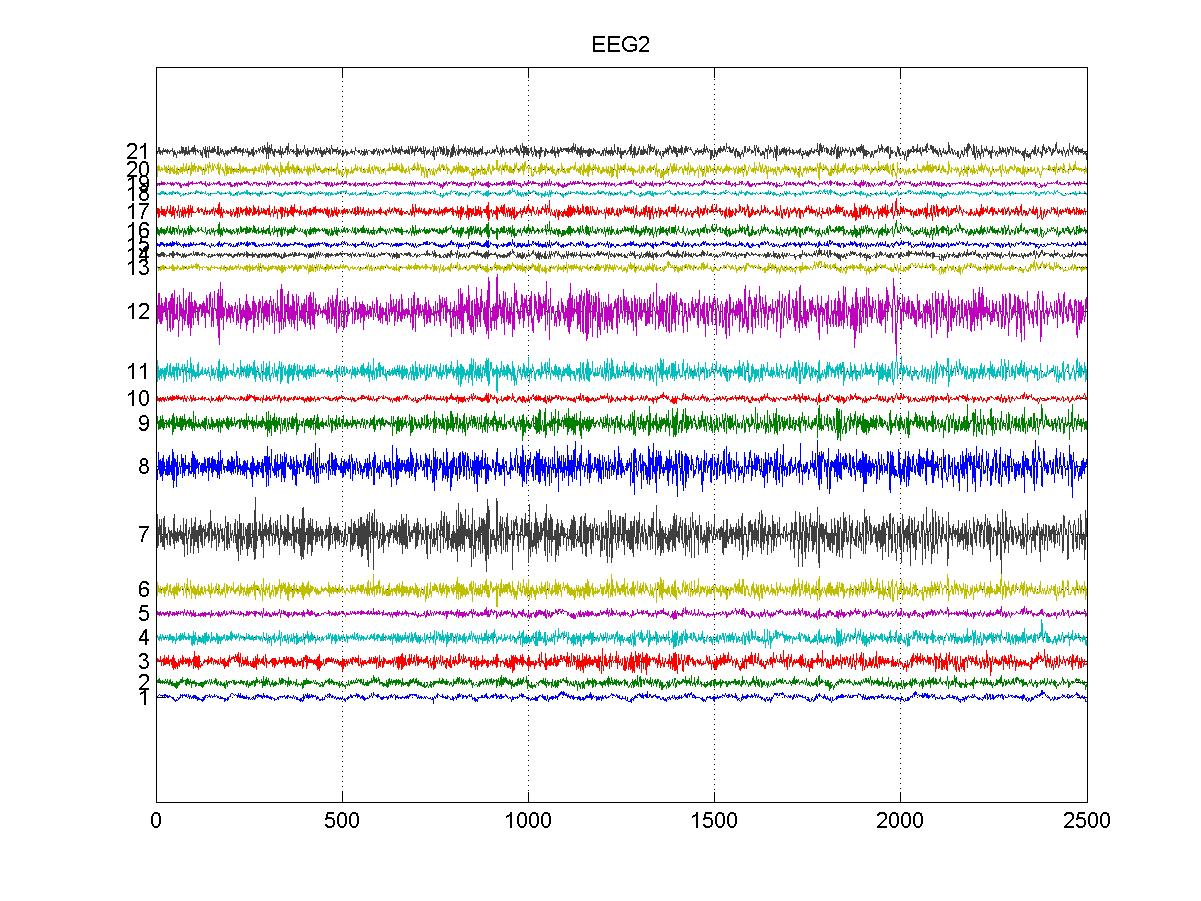
\includegraphics[width=.8\textwidth]{1.jpg}\\
\tiny{\tiny EEG signal of the first set}
\endminipage\hfill
\minipage{.5\textwidth}%
\centering
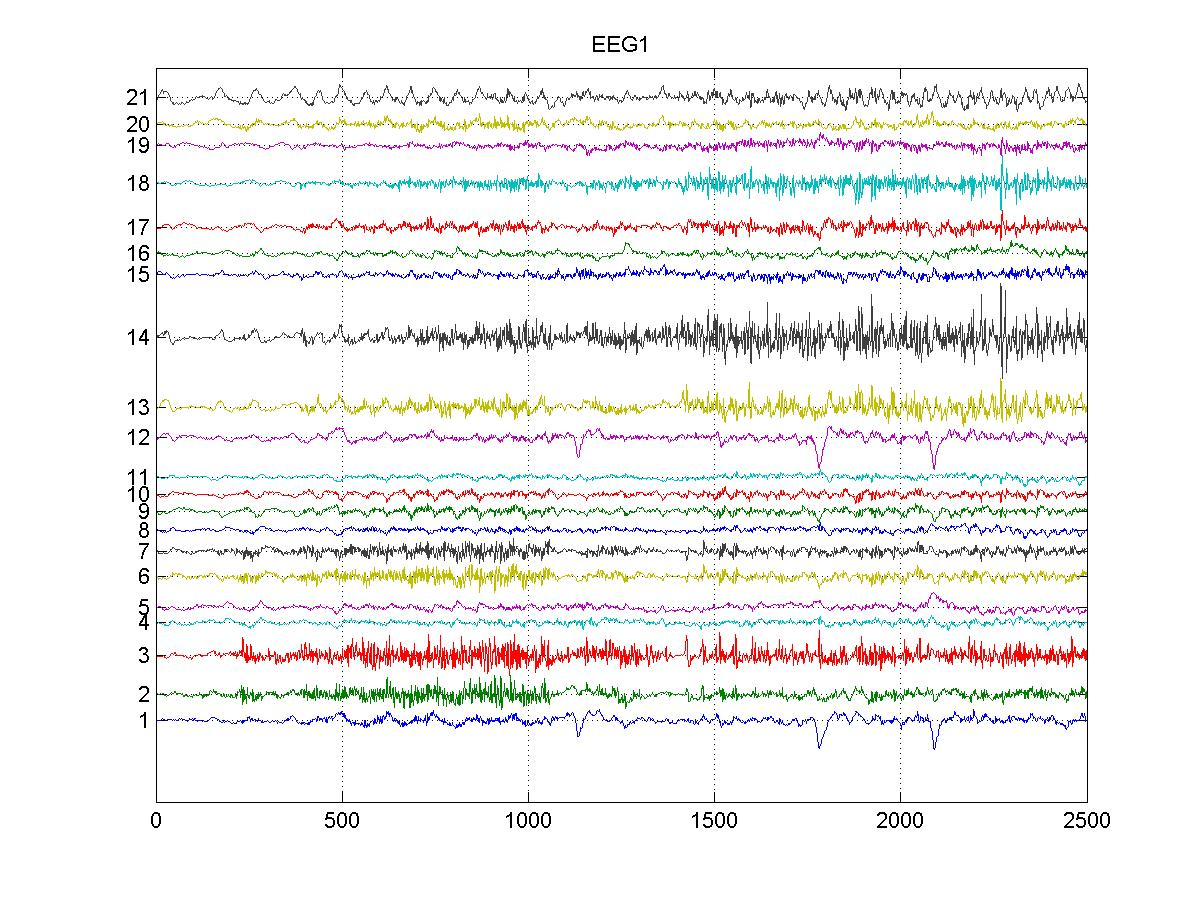
\includegraphics[width=.8\textwidth]{2.jpg}\\
\tiny{\tiny EEG signal of the second set}
\endminipage\hfill
\end{figure}

\tiny{Original EEG signals where in addition the most affected channels by the muscles artifacts are pointed out}

\end{frame}

\begin{frame}{CCA of the first set}

\begin{figure}[!htbp]
\minipage{.3\textwidth}%
\centering
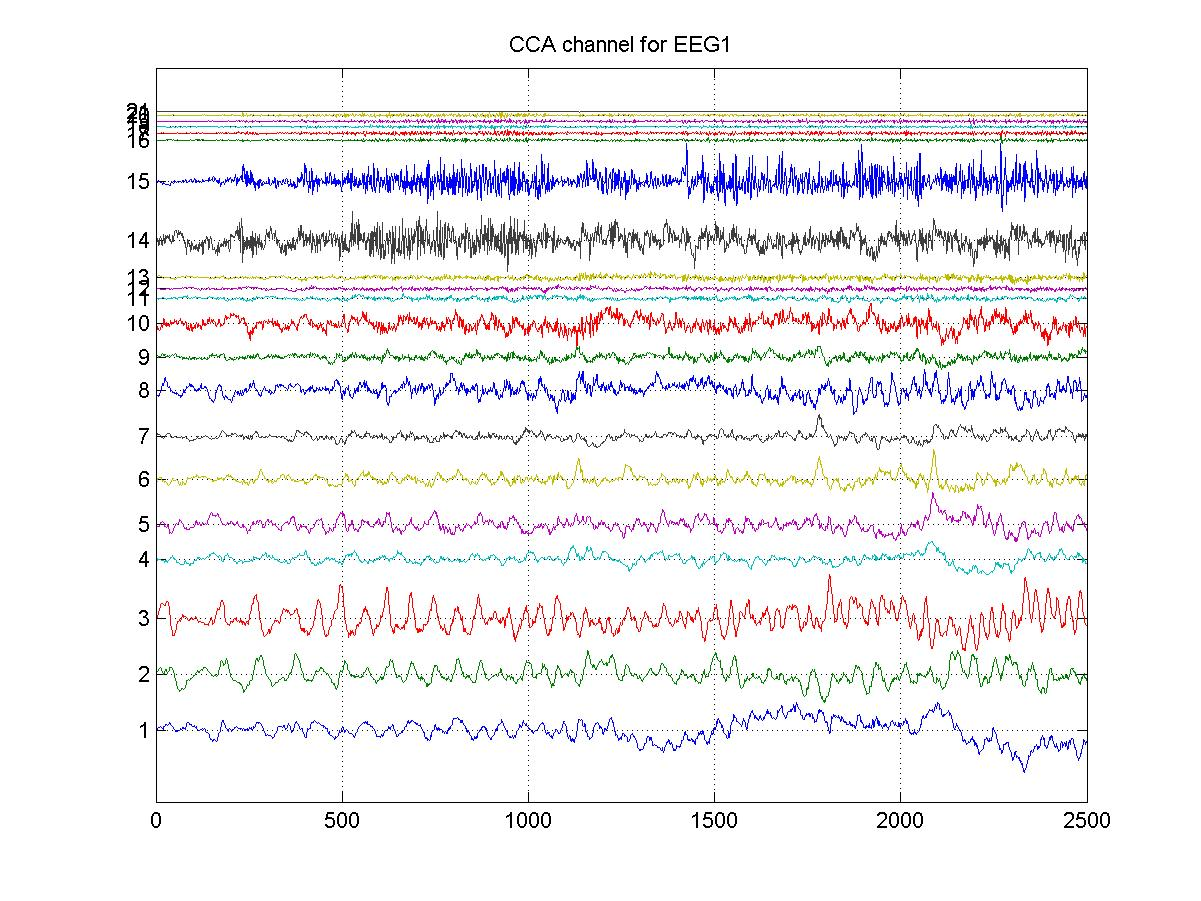
\includegraphics[width=1\textwidth]{3.jpg}\\
\tiny{\tiny EEG reconstructed signals after CCA}
\endminipage\hfill
\minipage{.3\textwidth}%
\centering
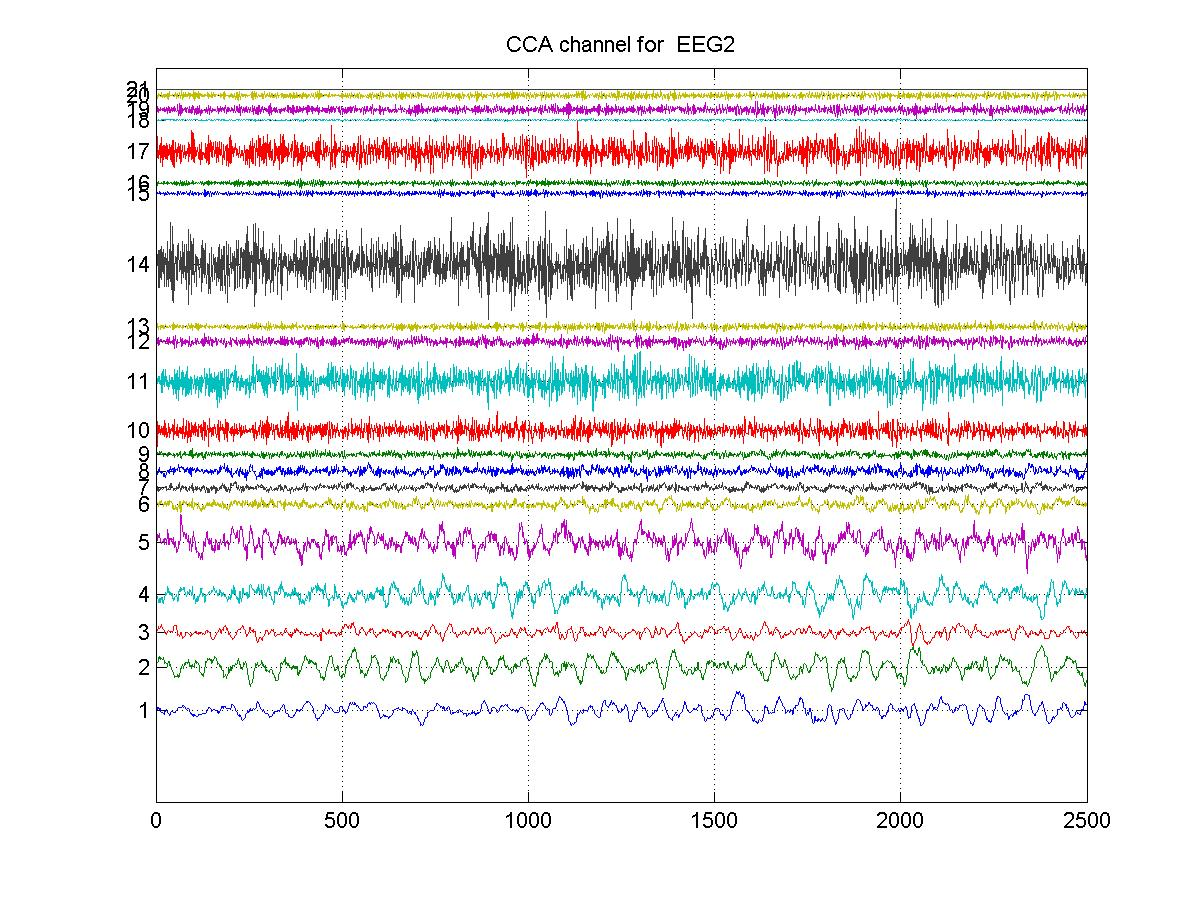
\includegraphics[width=1\textwidth]{4.jpg}\\
\tiny{\tiny The CCA source channel}
\endminipage\hfill
\minipage{.3\textwidth}%
\centering
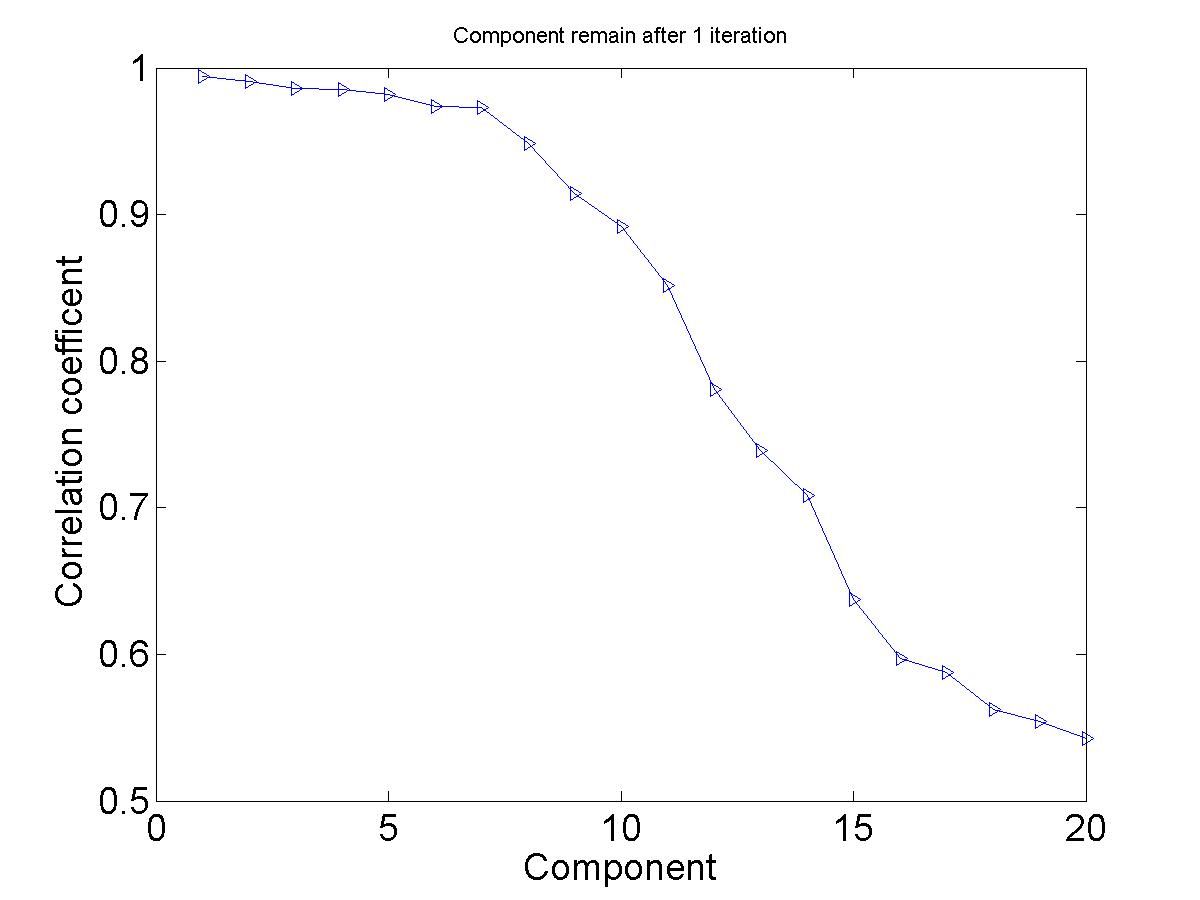
\includegraphics[width=1\textwidth]{5.jpg}\\
\tiny{\tiny Correlation values for respective channel}
\endminipage\hfill
\end{figure}

\begin{equation}
    EEG=W^{T}*CCA_{sources}
\end{equation}
 
\end{frame} 
      
    
\begin{frame}{CCA of the second set}

\begin{figure}[!htbp]
\minipage{.3\textwidth}%
\centering
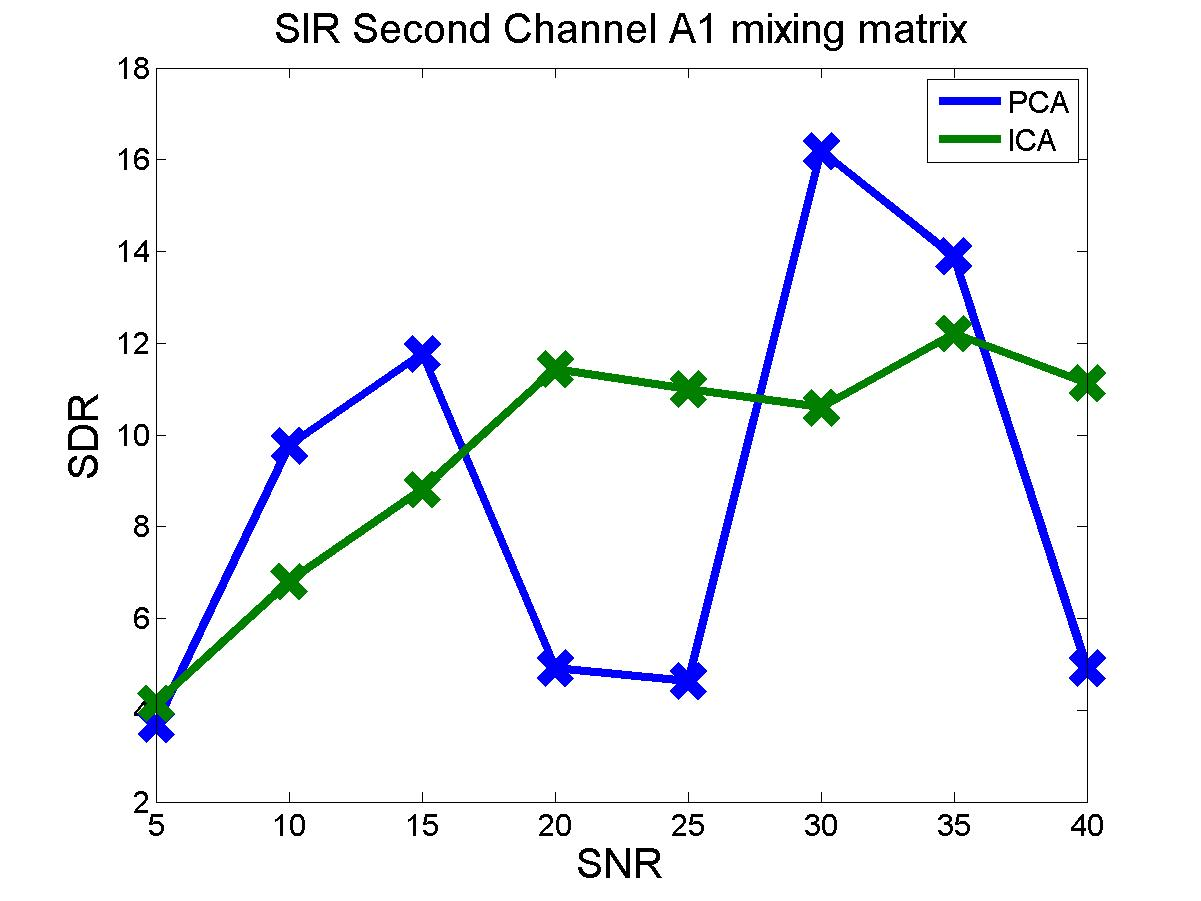
\includegraphics[width=1\textwidth]{6.jpg}\\
\tiny{EEG reconstructed signals after CCA}
\endminipage\hfill
\minipage{.3\textwidth}%
\centering
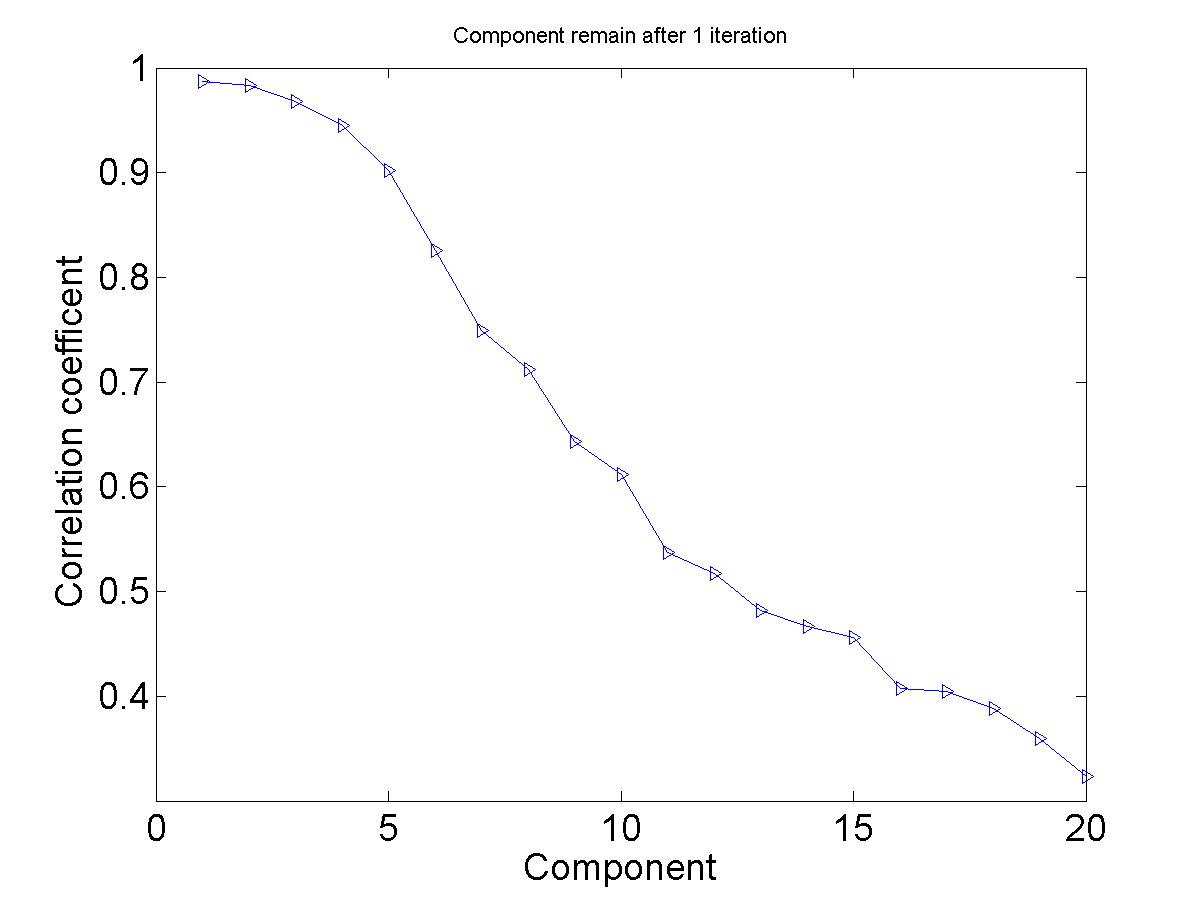
\includegraphics[width=1\textwidth]{7.jpg}\\
\tiny{The CCA source channel}
\endminipage\hfill
\minipage{.3\textwidth}%
\centering
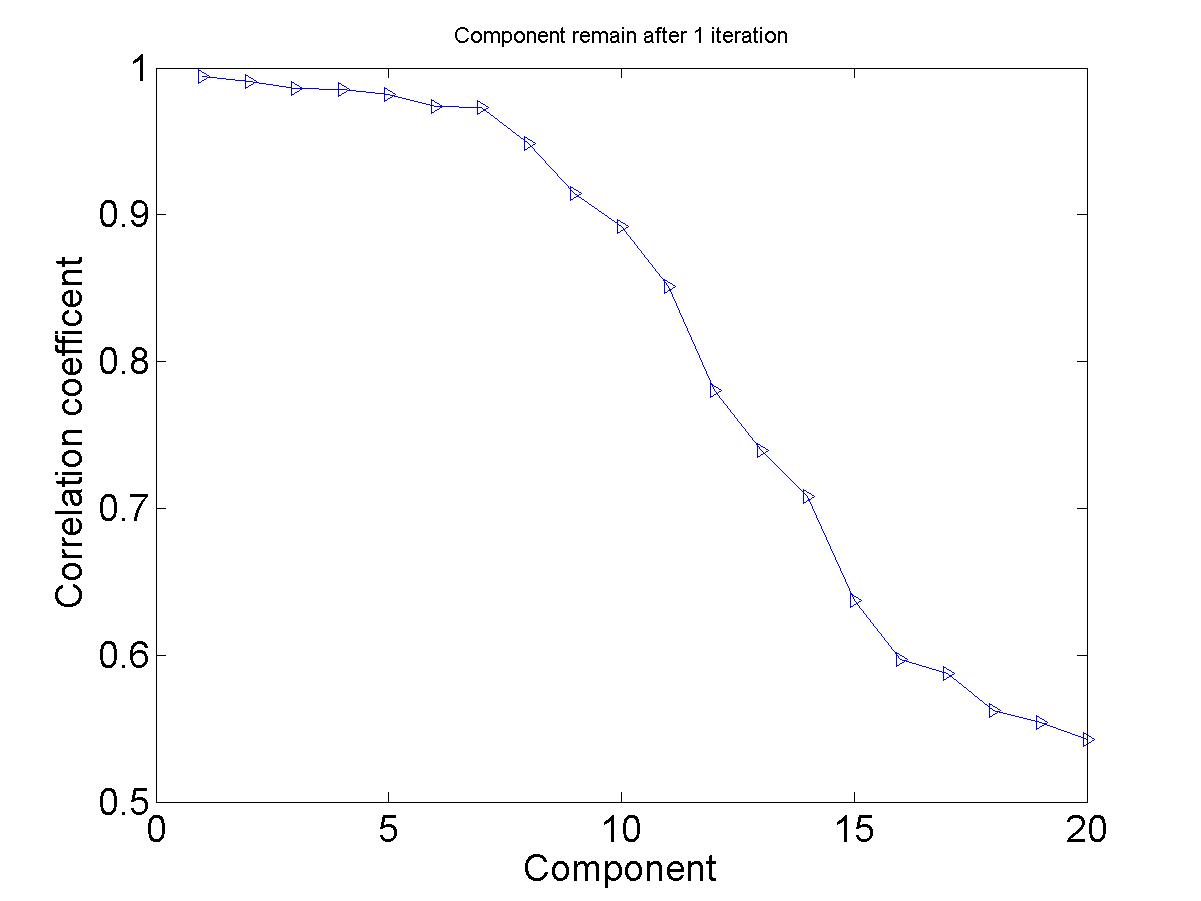
\includegraphics[width=1\textwidth]{8.jpg}\\
\tiny{Correlation values for respective channel}
\endminipage\hfill
\end{figure}

\begin{equation}
    EEG=W^{T}*CCA_{sources}
\end{equation}

\end{frame} 
    
    
\begin{frame}{Manual processing  for the first set}

\begin{figure}[!htbp]
\minipage{.3\textwidth}%
\centering
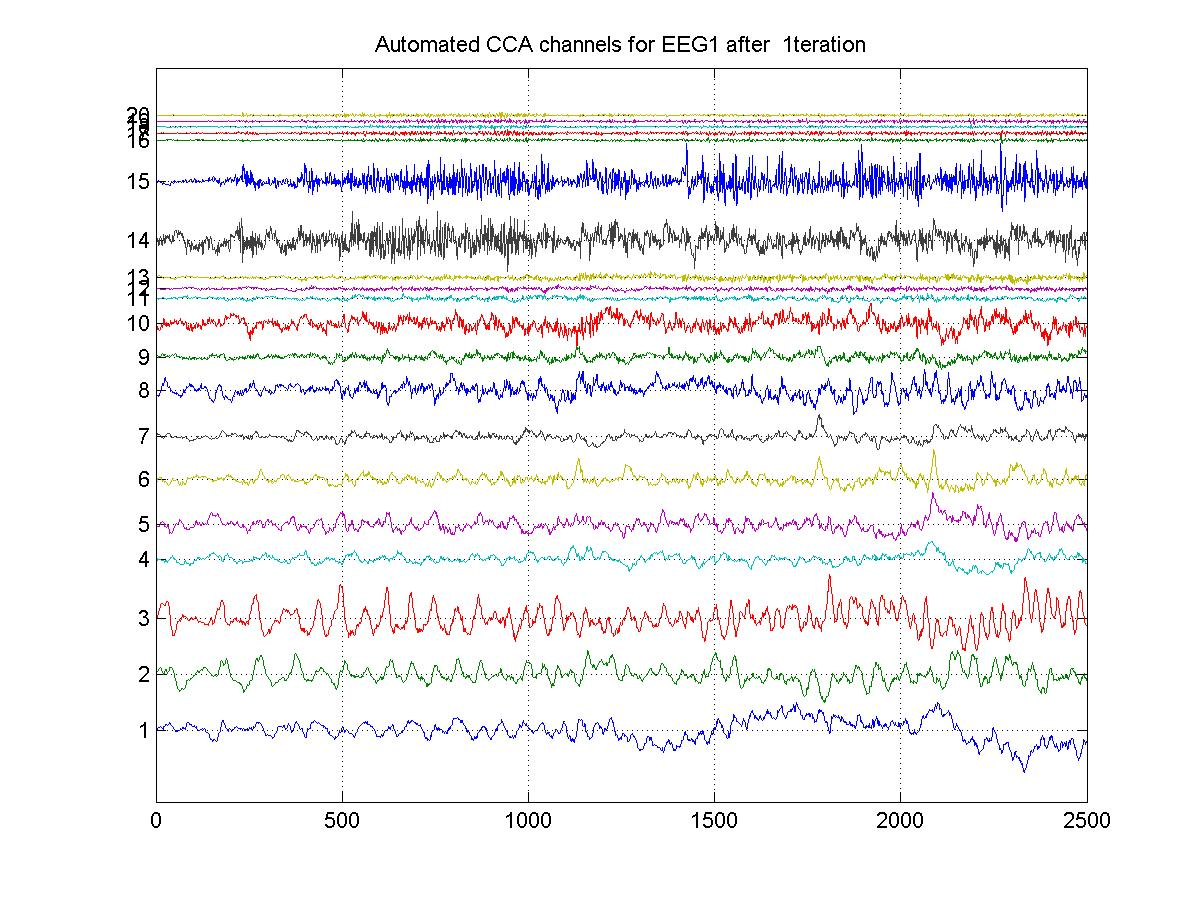
\includegraphics[width=1\textwidth]{9.jpg}\\
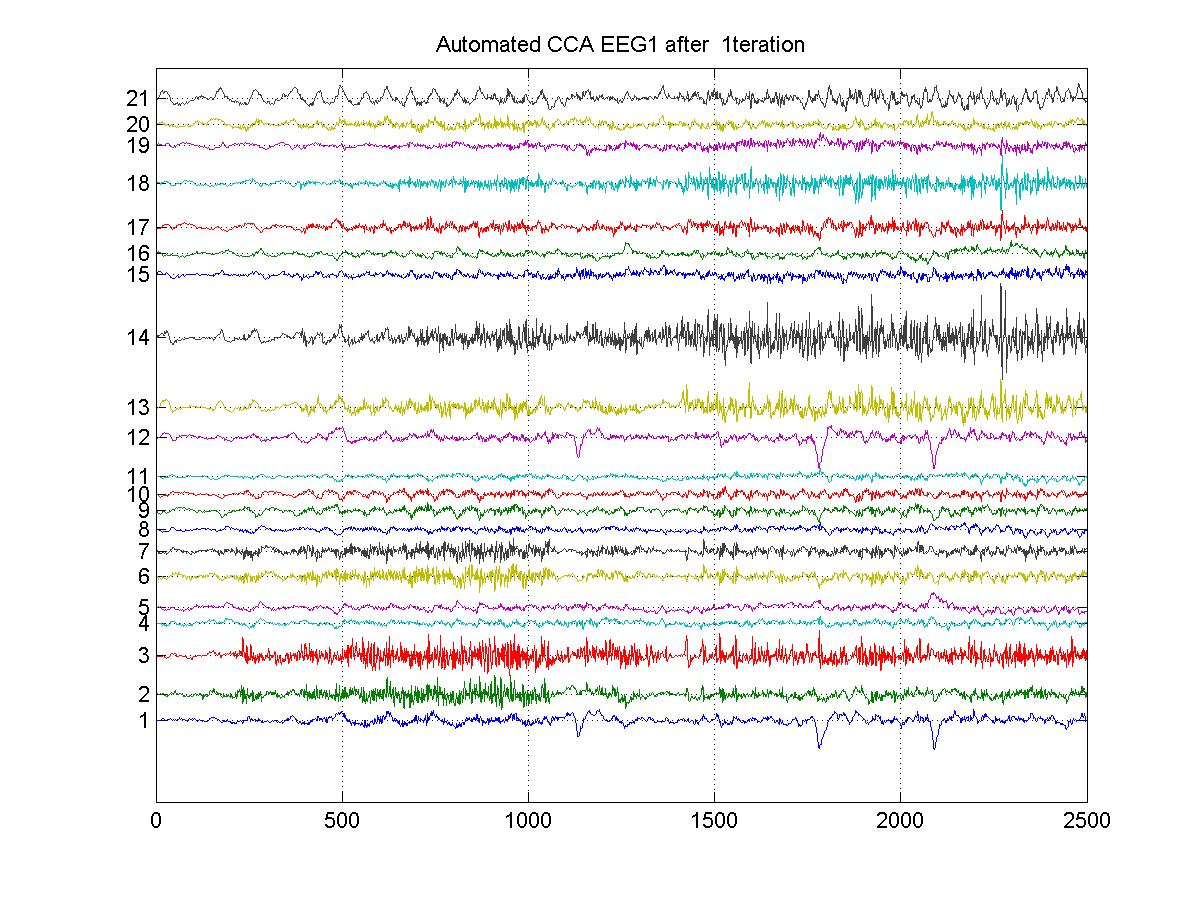
\includegraphics[width=1\textwidth]{10.jpg}
\endminipage\hfill
\minipage{.3\textwidth}%
\centering
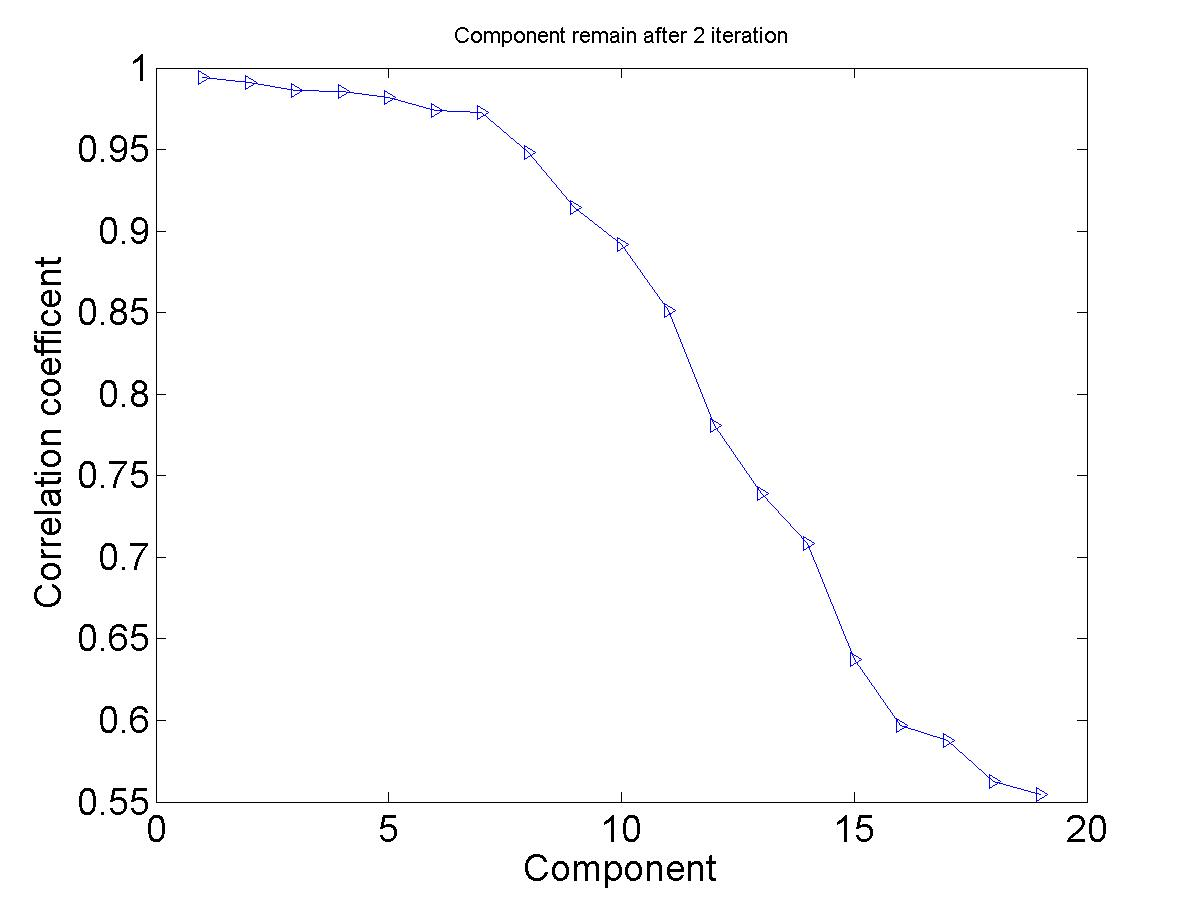
\includegraphics[width=1\textwidth]{11.jpg}\\
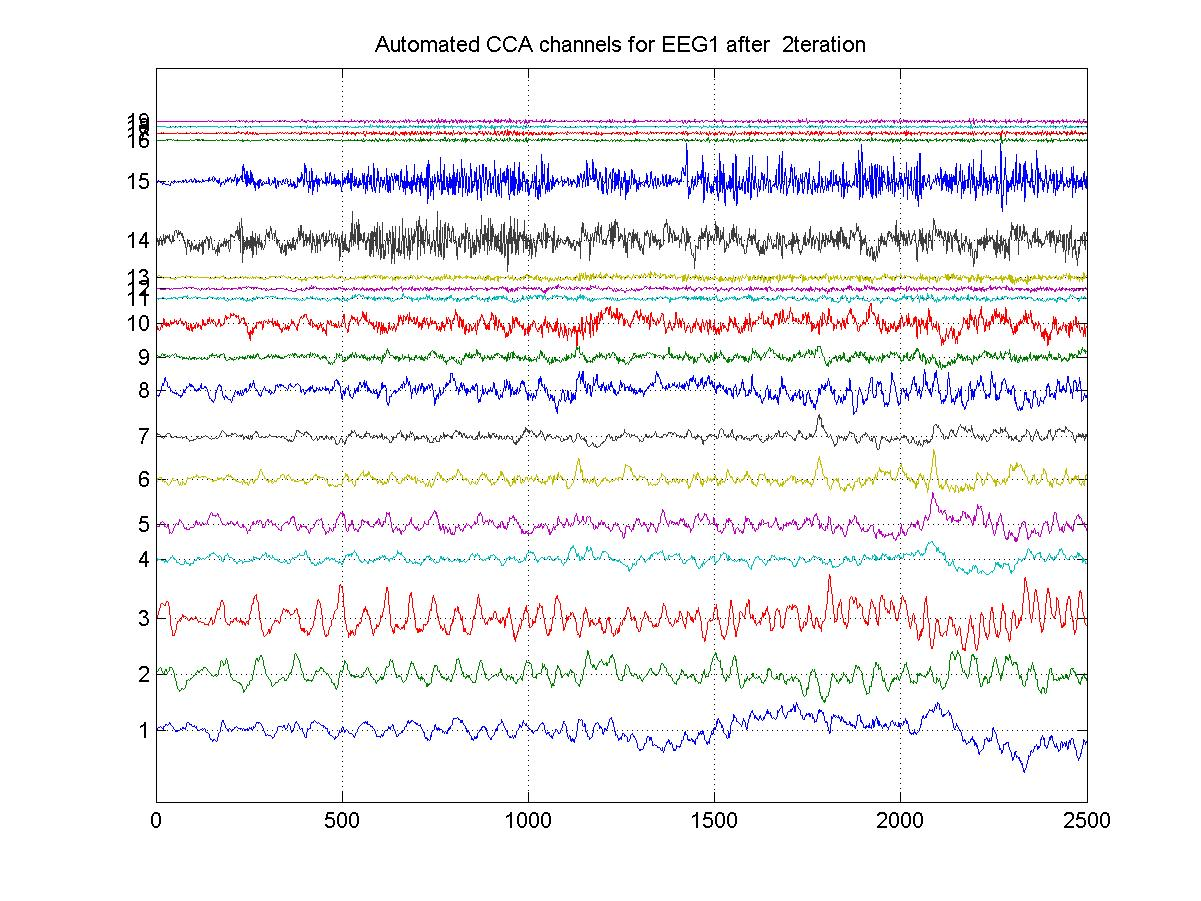
\includegraphics[width=1\textwidth]{12.jpg}
\endminipage\hfill
\minipage{.3\textwidth}%
\centering
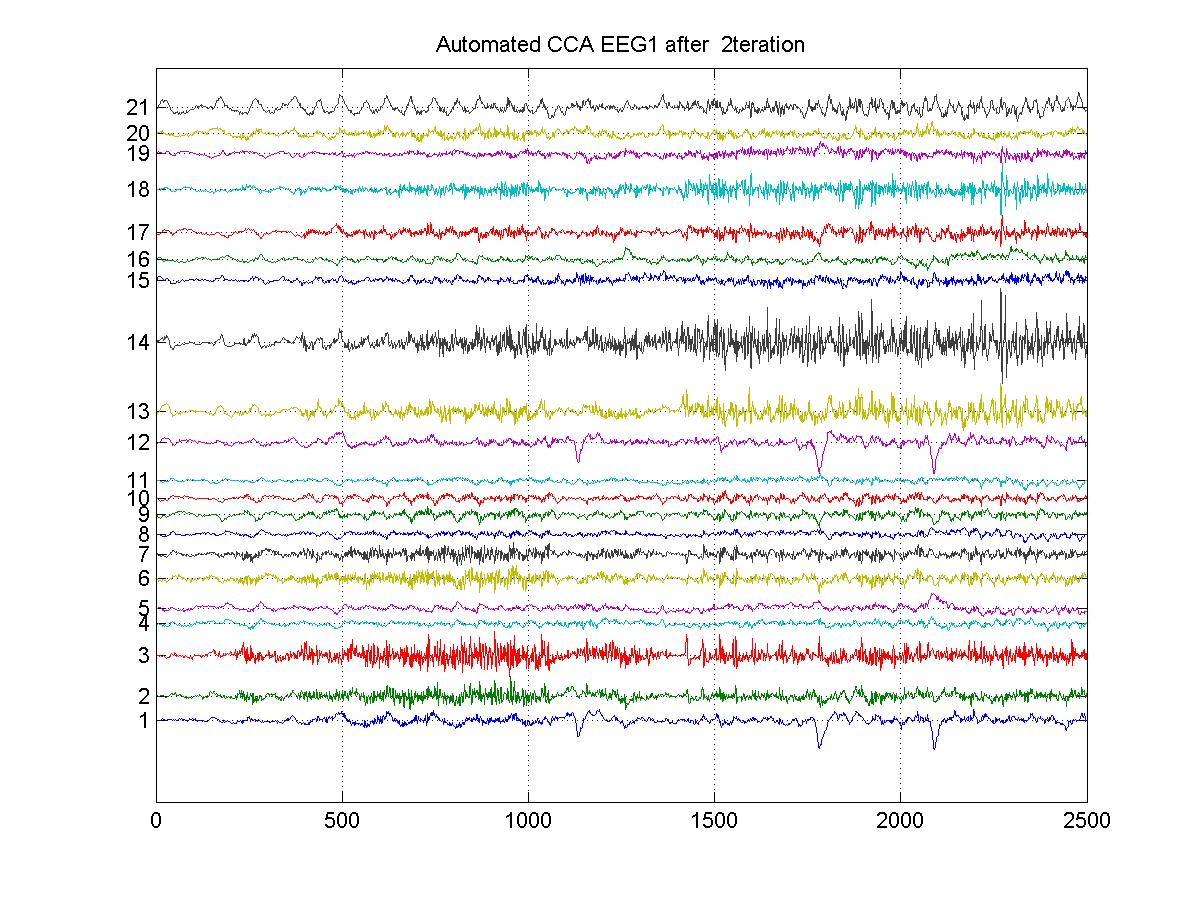
\includegraphics[width=1\textwidth]{13.jpg}\\
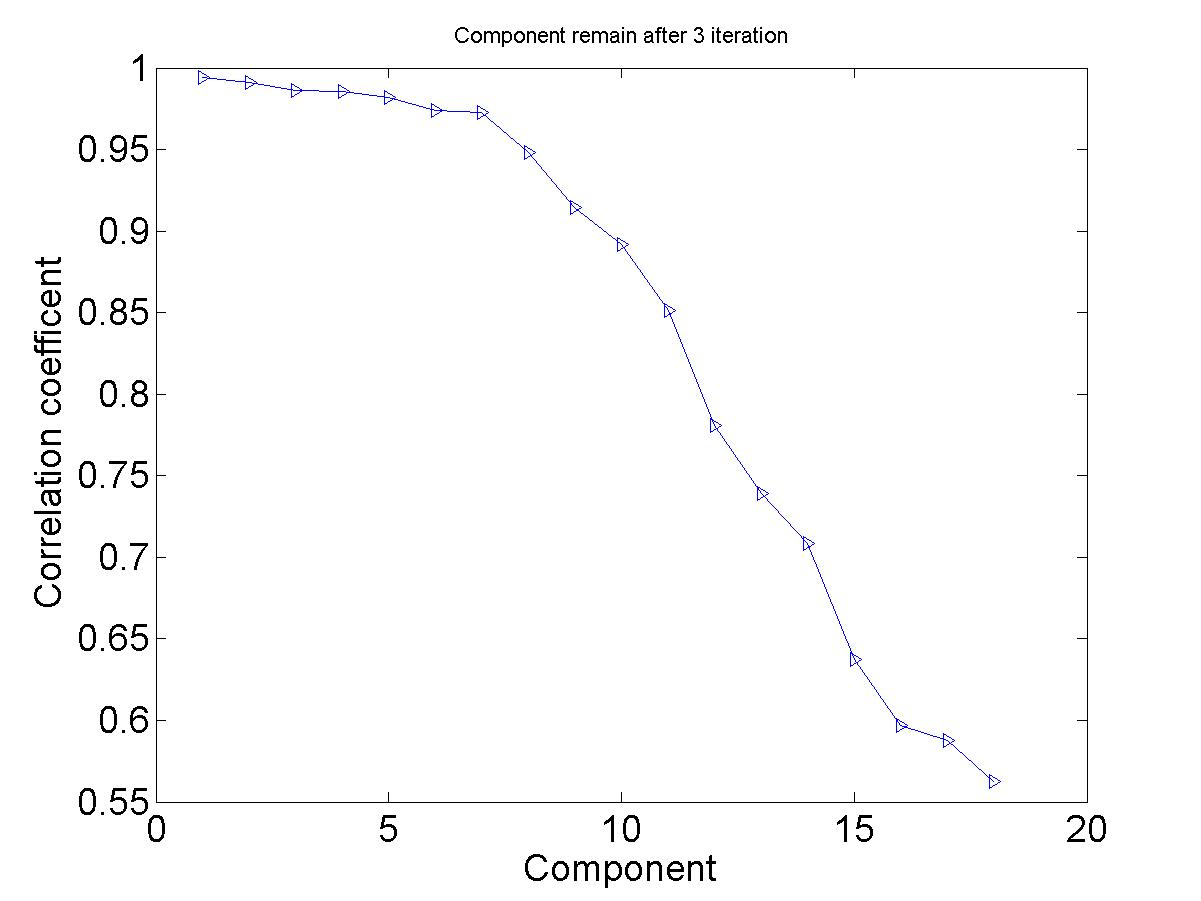
\includegraphics[width=1\textwidth]{14.jpg}
\endminipage\hfill
\end{figure}
  
\end{frame}  
    
\begin{frame}{Manual processing  for the second set}

\begin{figure}[!htbp]
\minipage{.3\textwidth}%
\centering
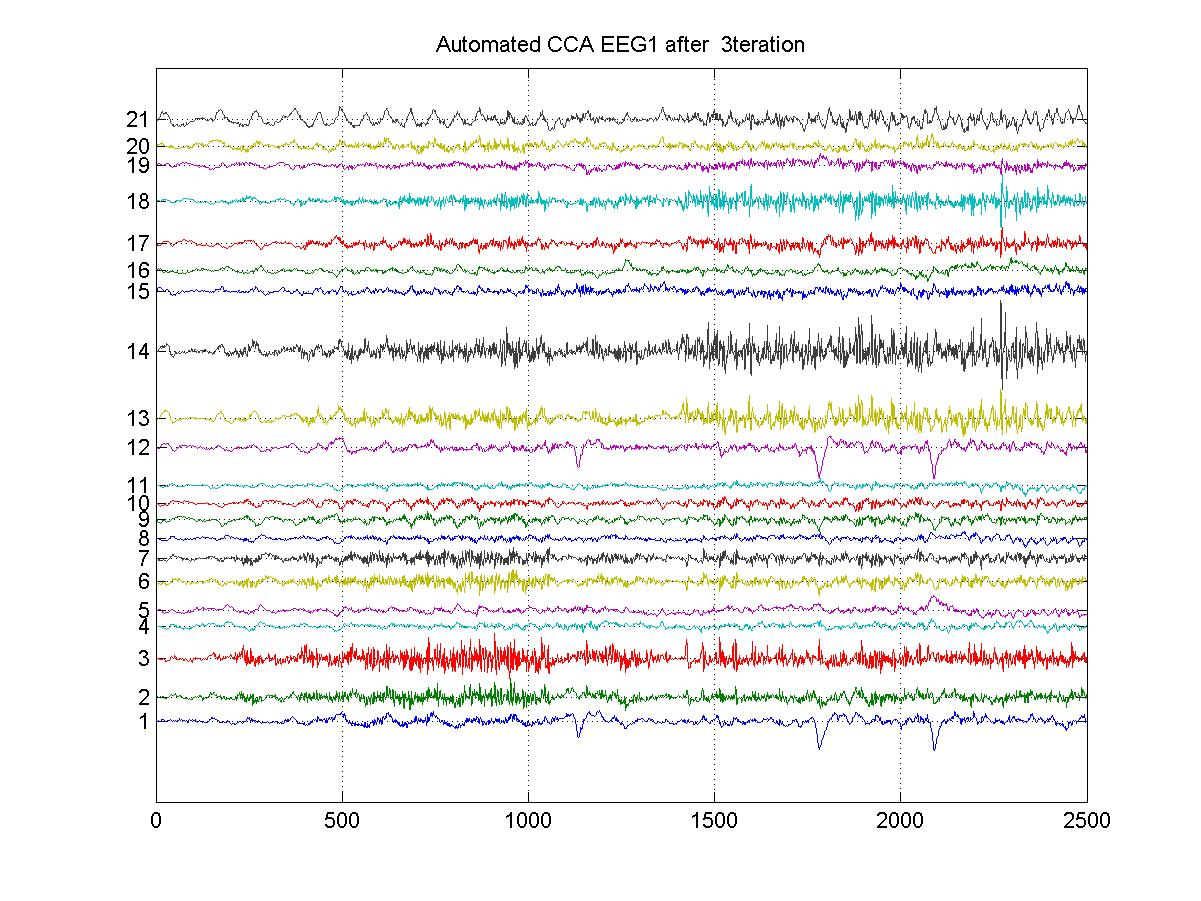
\includegraphics[width=1\textwidth]{16.jpg}\\
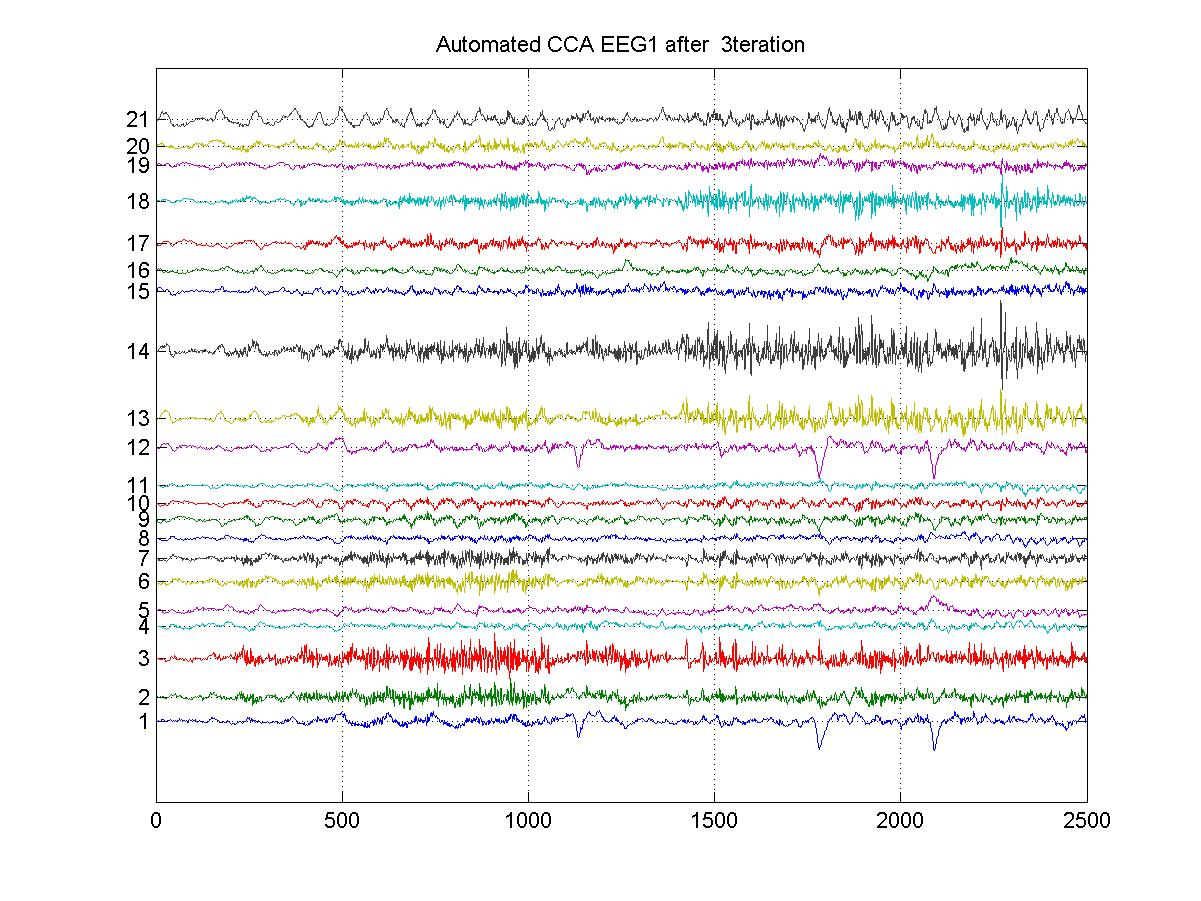
\includegraphics[width=1\textwidth]{16.jpg}
\endminipage\hfill
\minipage{.3\textwidth}%
\centering
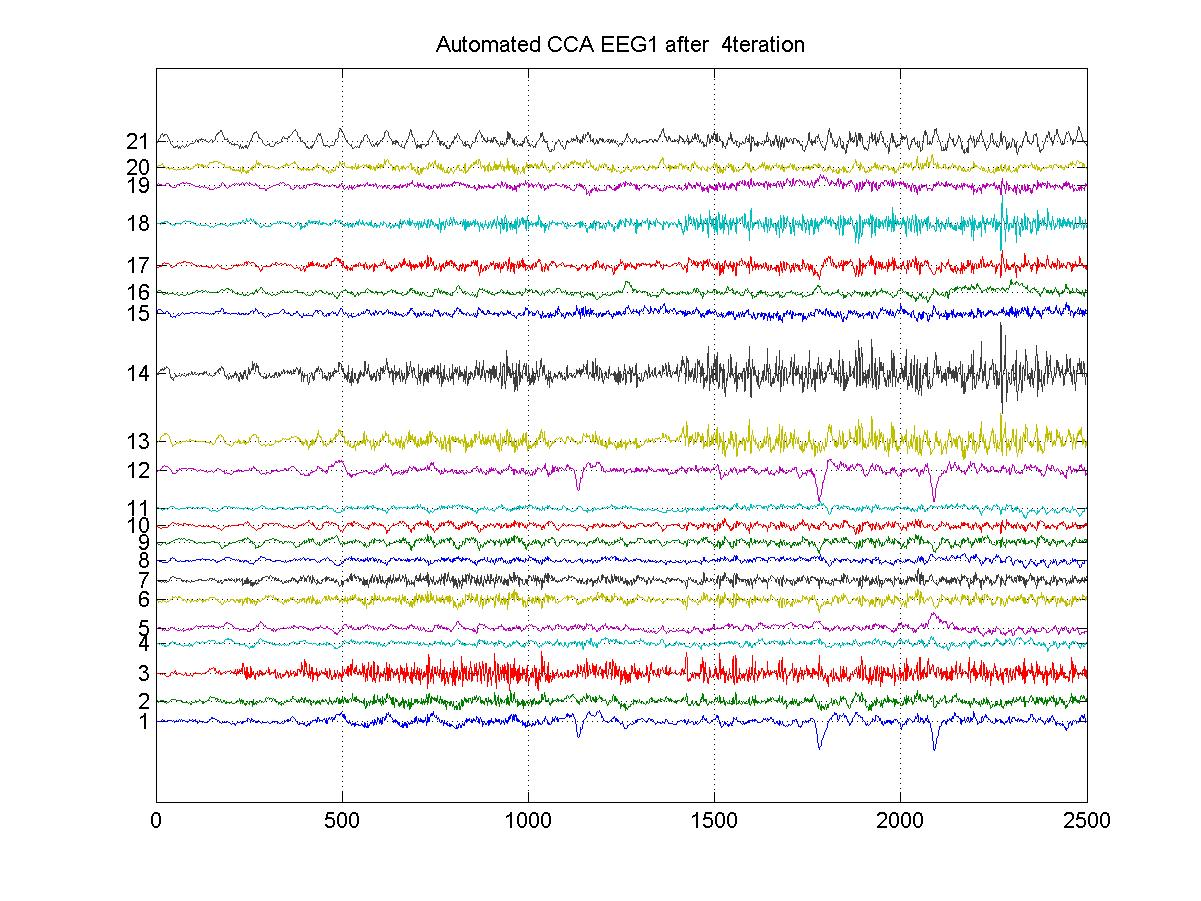
\includegraphics[width=1\textwidth]{19.jpg}\\
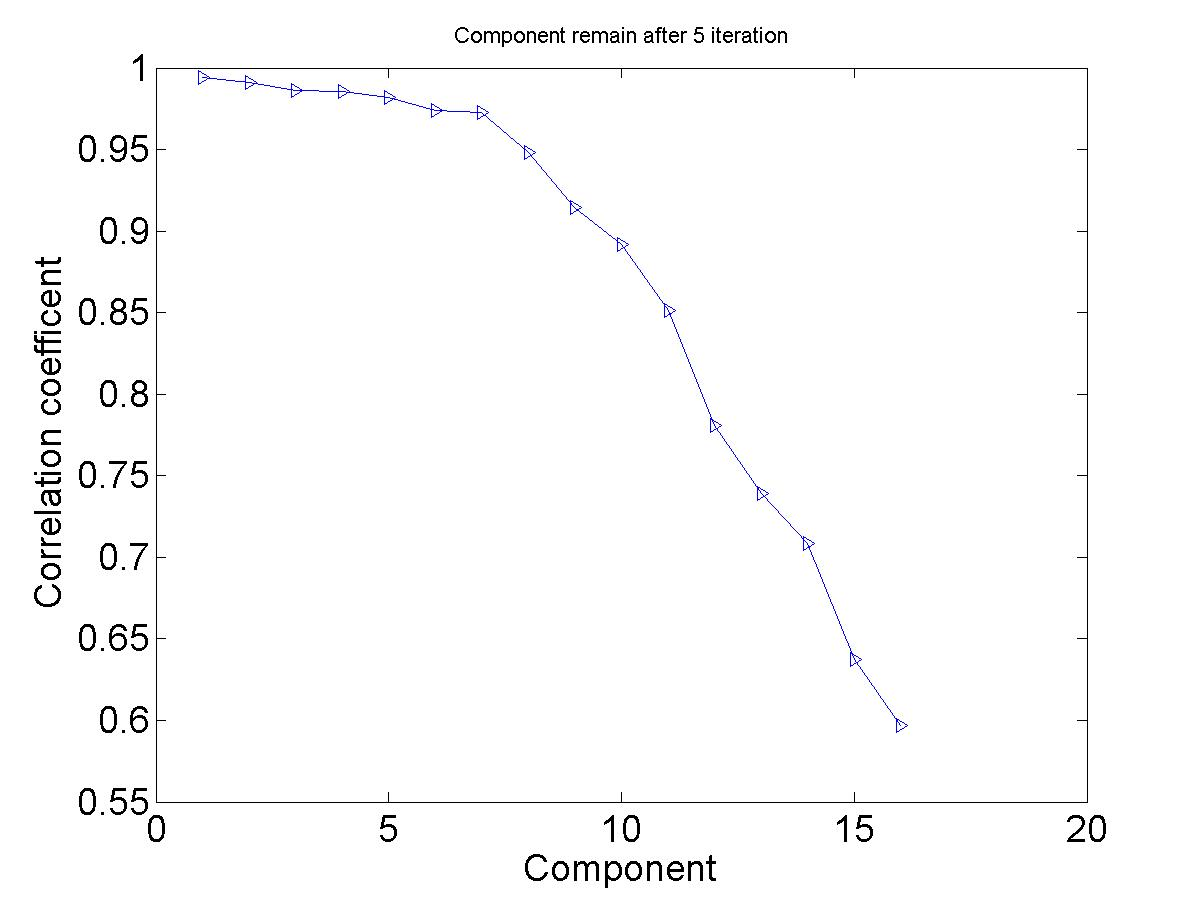
\includegraphics[width=1\textwidth]{20.jpg}
\endminipage\hfill
\minipage{.3\textwidth}%
\centering
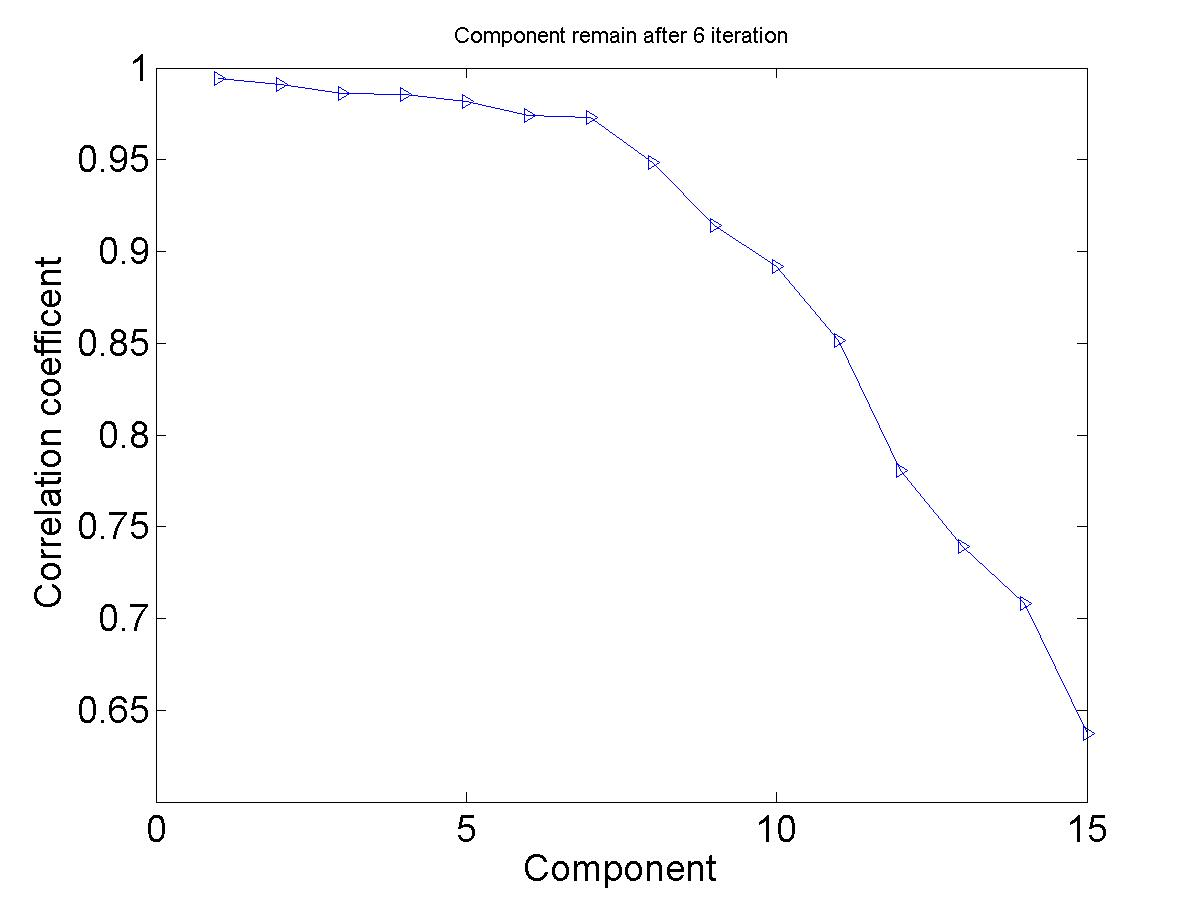
\includegraphics[width=1\textwidth]{23.jpg}\\
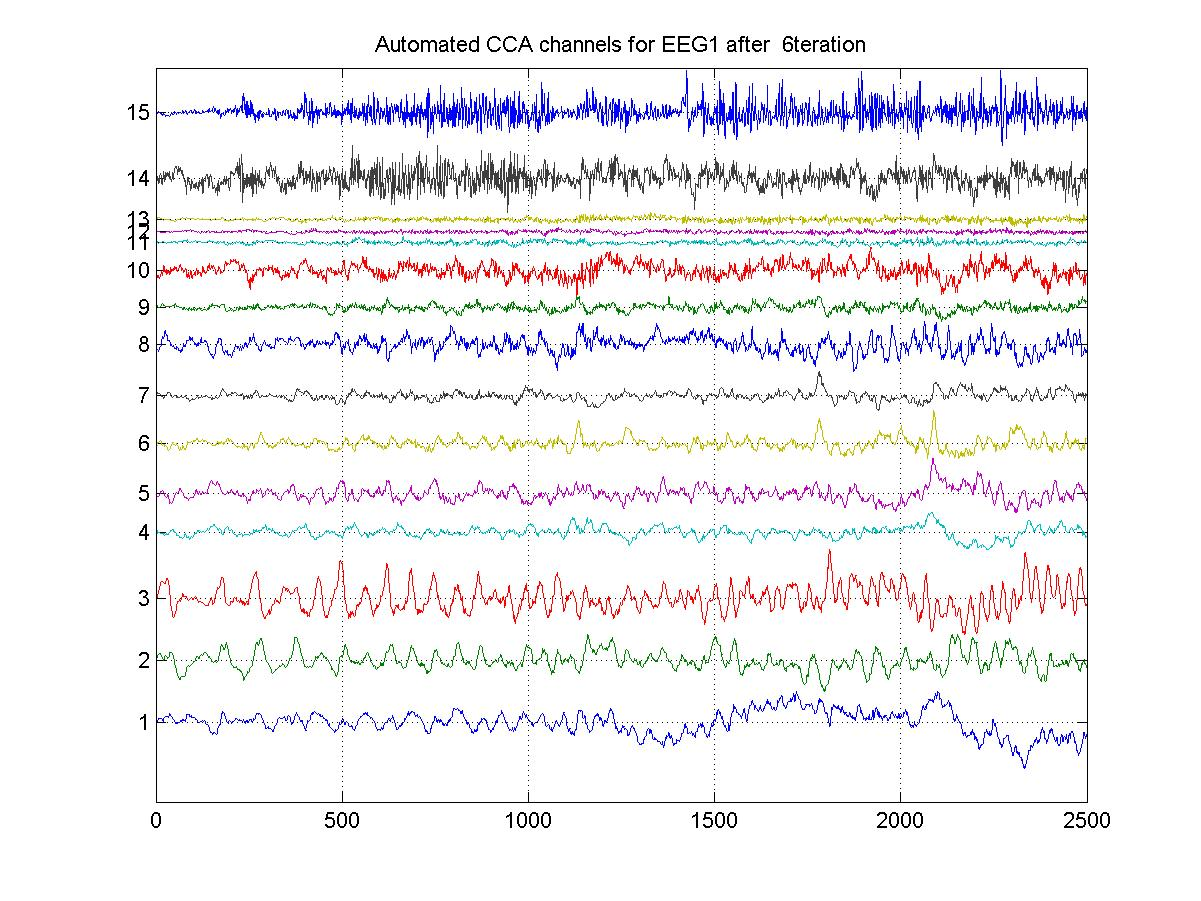
\includegraphics[width=1\textwidth]{24.jpg}
\endminipage\hfill
\end{figure}

 
\end{frame}  

\begin{frame}{Manual processing  for the second set \textit{.cont}}

\begin{figure}[!htbp]
\minipage{.3\textwidth}%
\centering
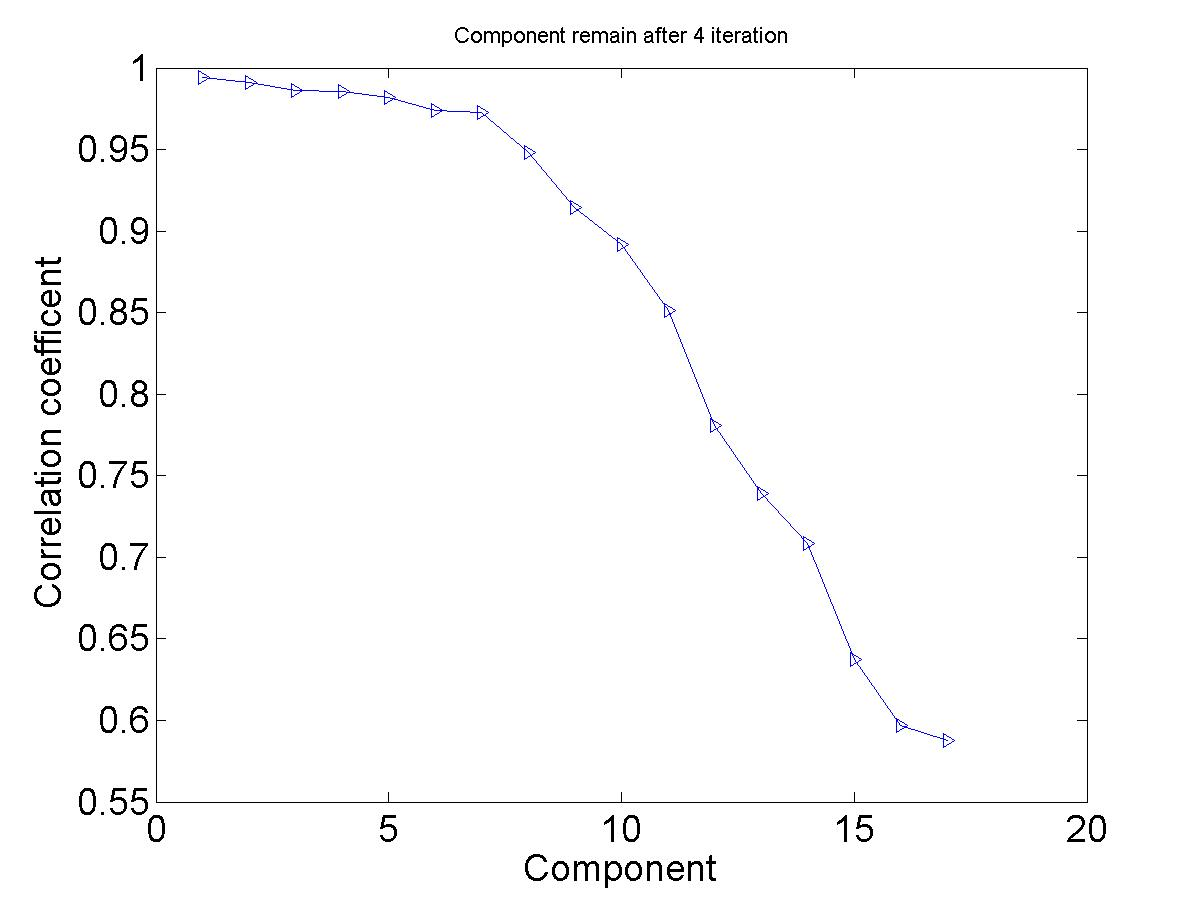
\includegraphics[width=1\textwidth]{17.jpg}\\
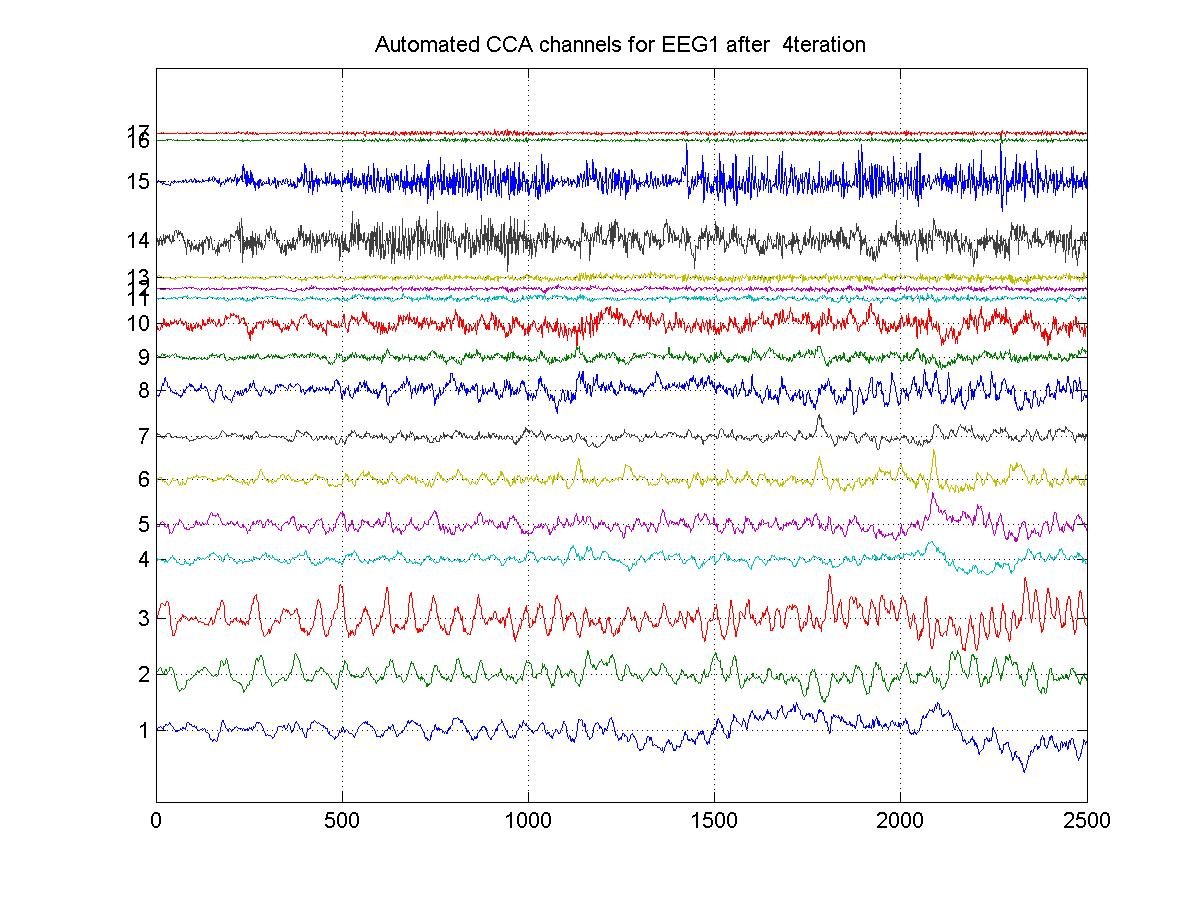
\includegraphics[width=1\textwidth]{18.jpg}
\endminipage\hfill
\minipage{.3\textwidth}%
\centering
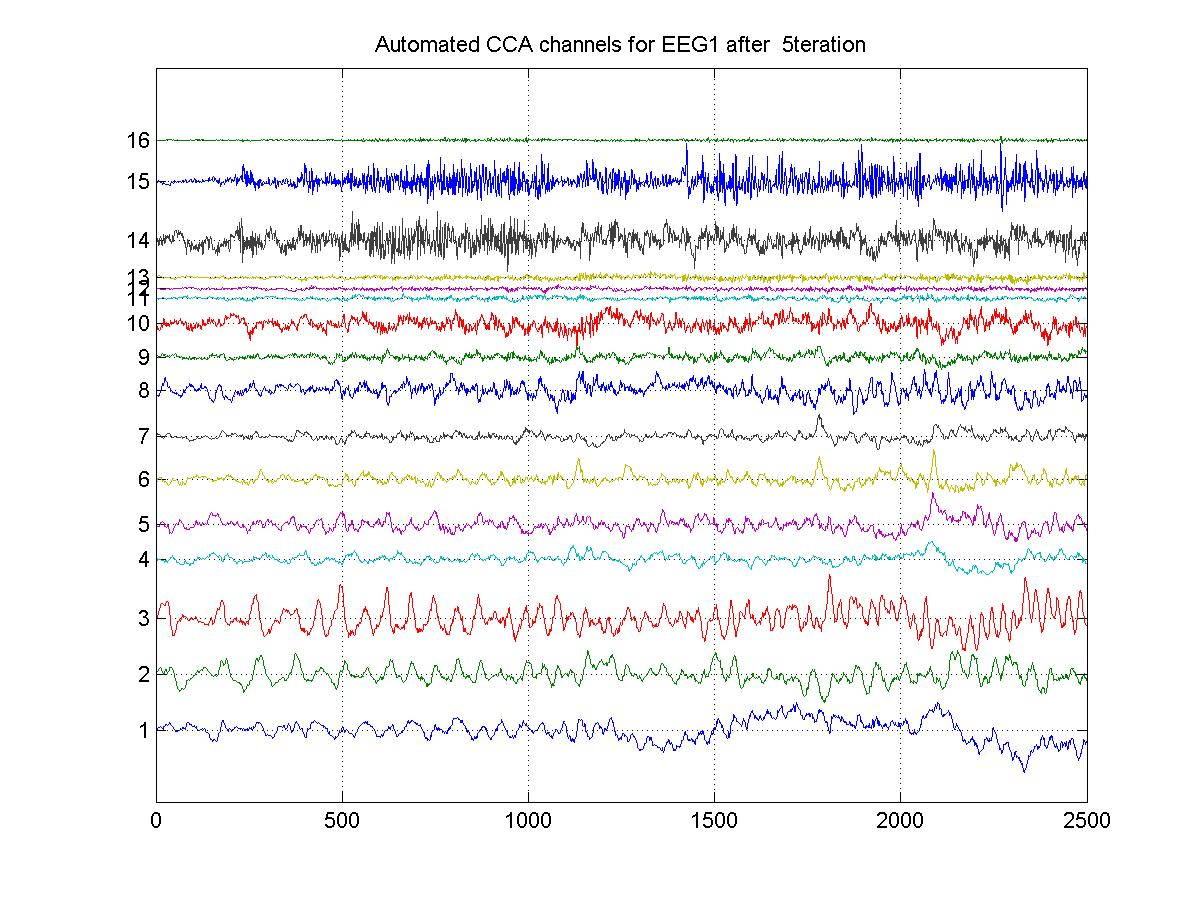
\includegraphics[width=1\textwidth]{21.jpg}\\
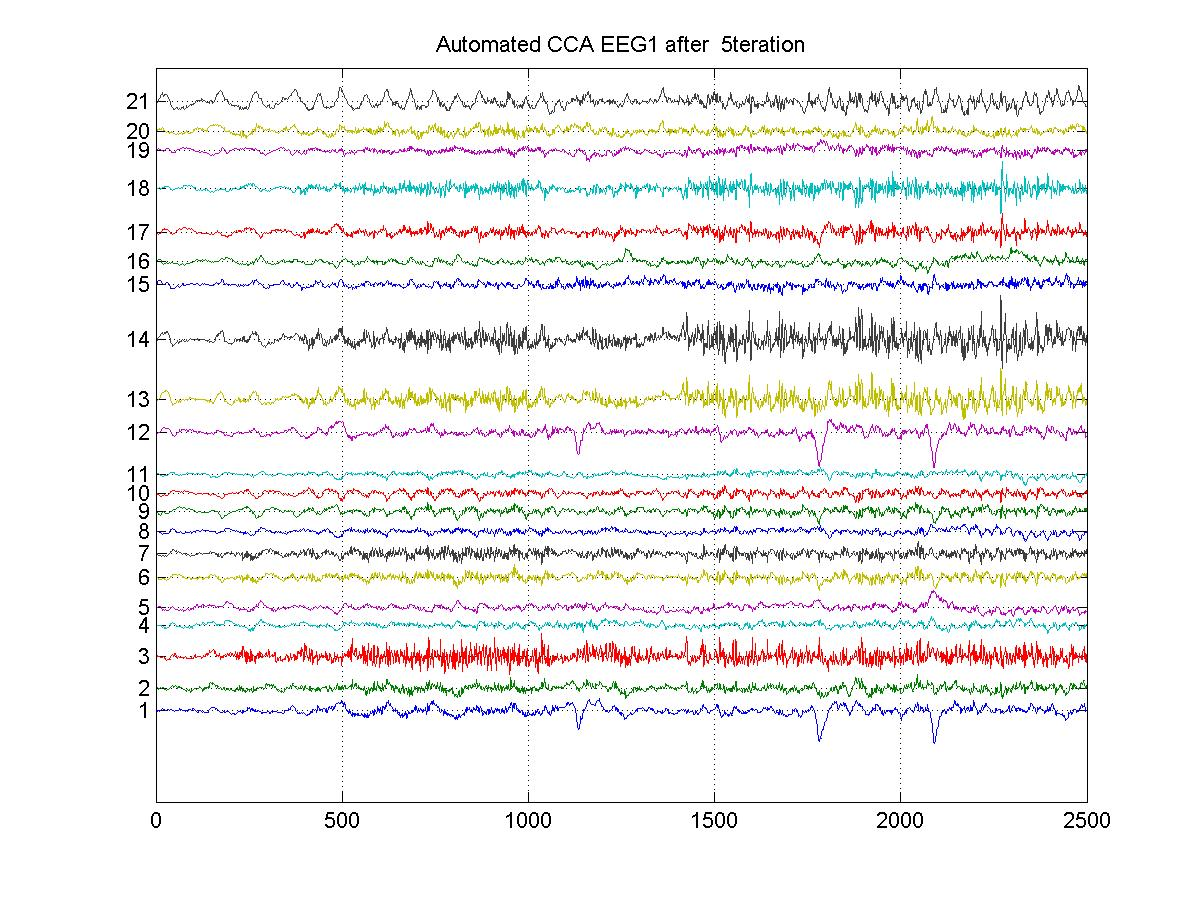
\includegraphics[width=1\textwidth]{22.jpg}
\endminipage\hfill
\minipage{.3\textwidth}%
\centering
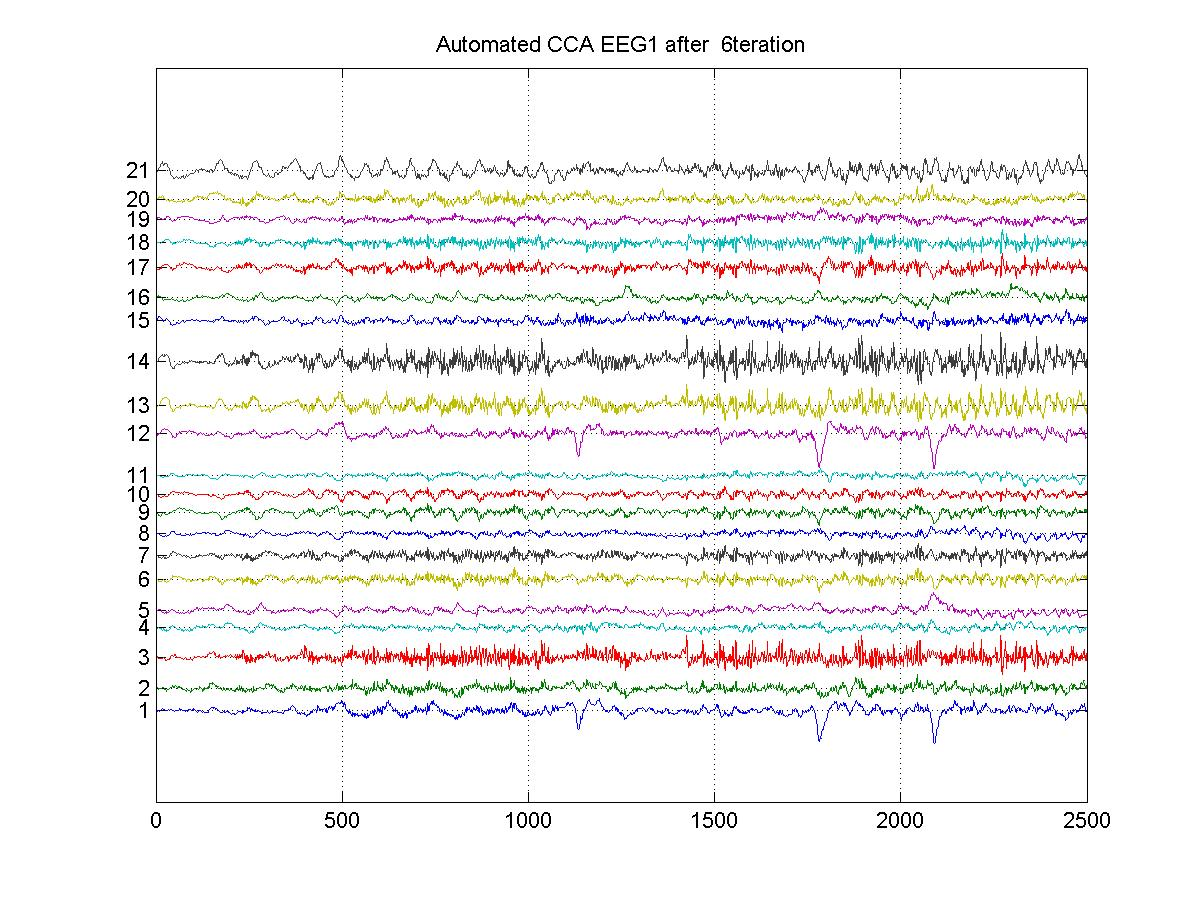
\includegraphics[width=1\textwidth]{25.jpg}\\
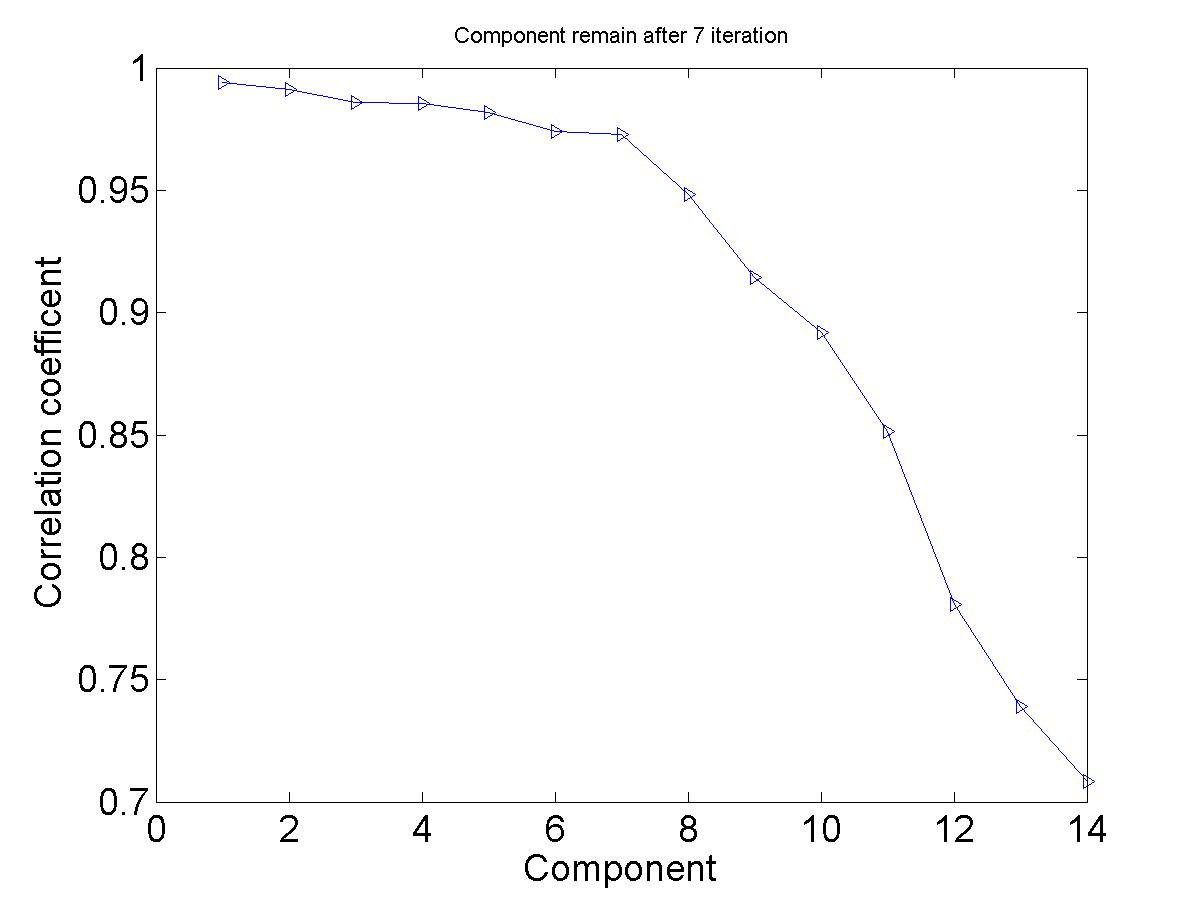
\includegraphics[width=1\textwidth]{26.jpg}
\endminipage\hfill
\end{figure}

 
\end{frame}  
 
 
 
\begin{frame}{Automated processing for the second set }


\begin{figure}[!htbp]
\minipage{.5\textwidth}%
\centering
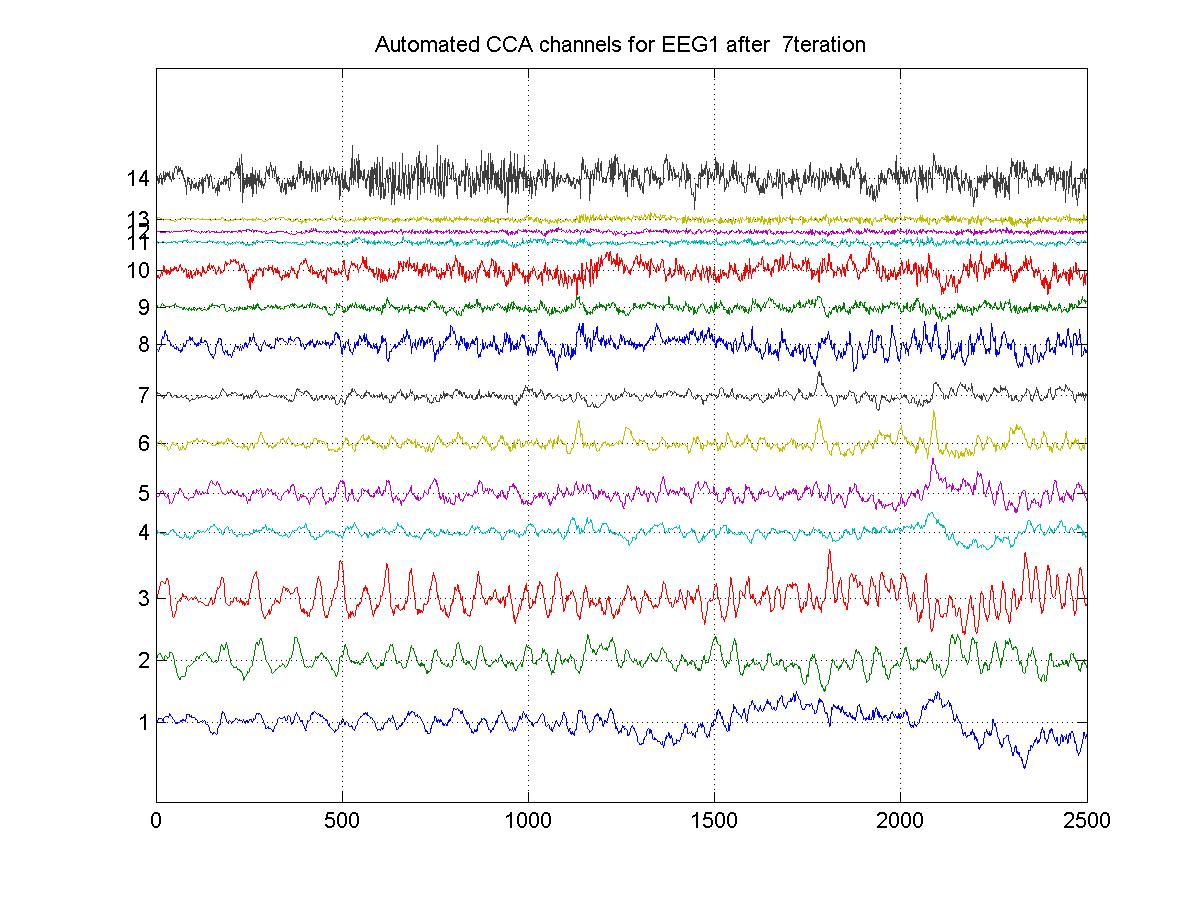
\includegraphics[width=.8\textwidth]{27.jpg}\\
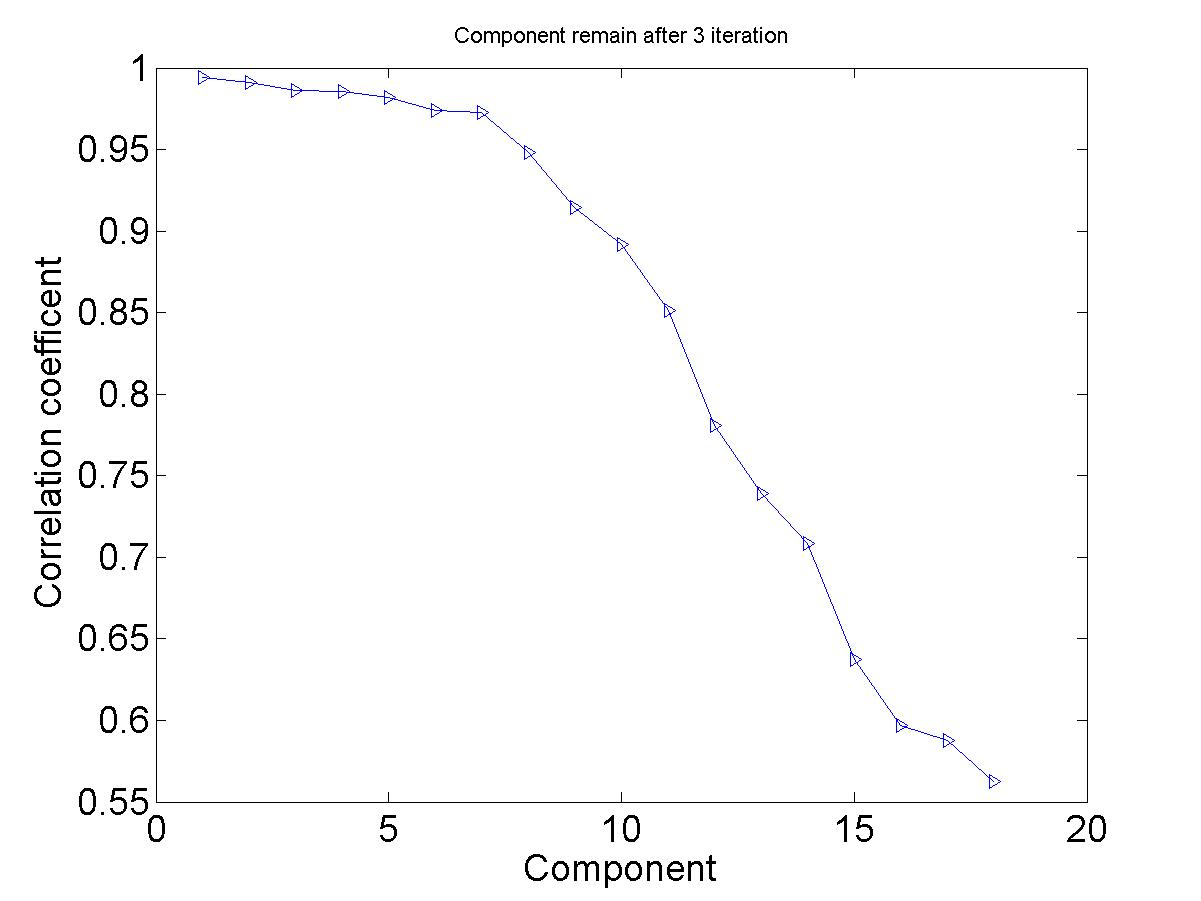
\includegraphics[width=.8\textwidth]{14.jpg}\\
\tiny{CCA results of the first data set}\label{toda1}
\endminipage\hfill
\minipage{.5\textwidth}%
\centering
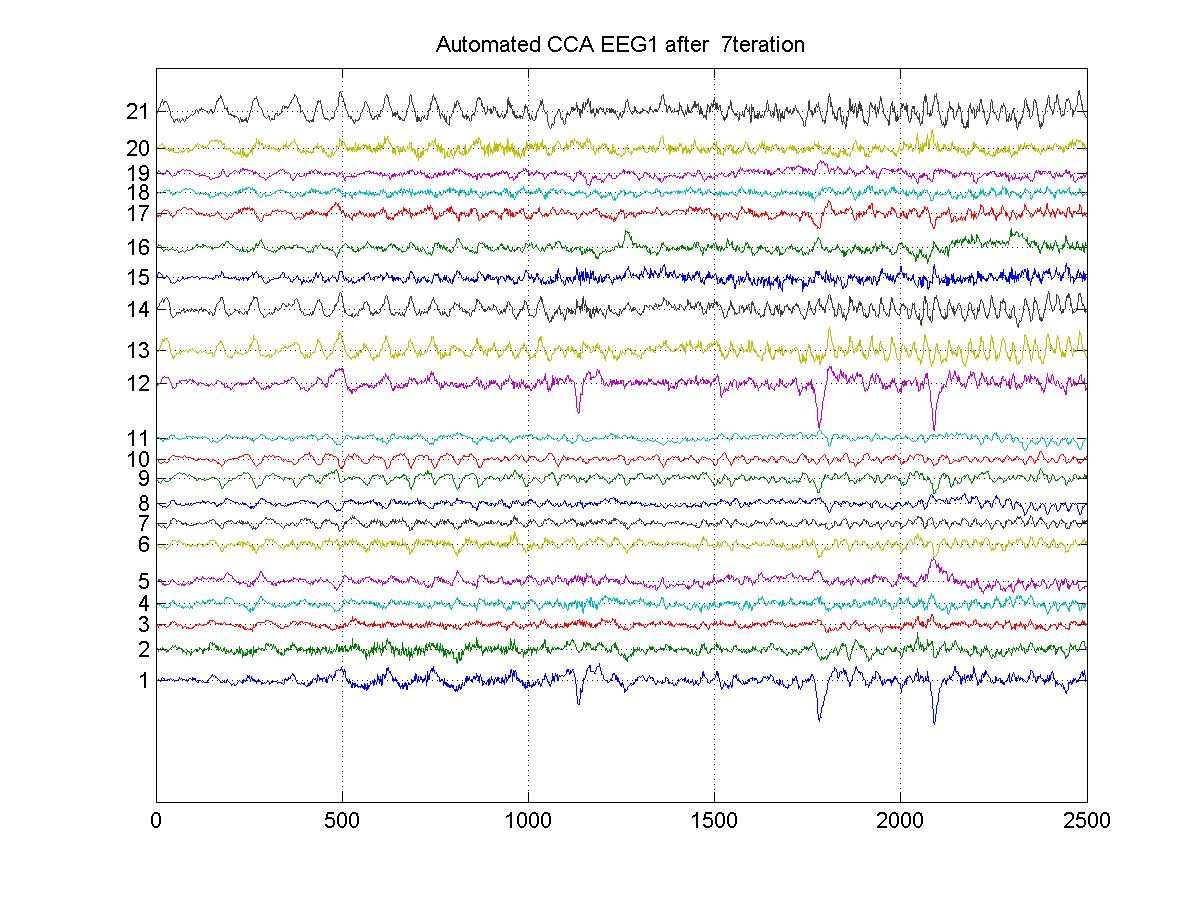
\includegraphics[width=.8\textwidth]{28.jpg}\\
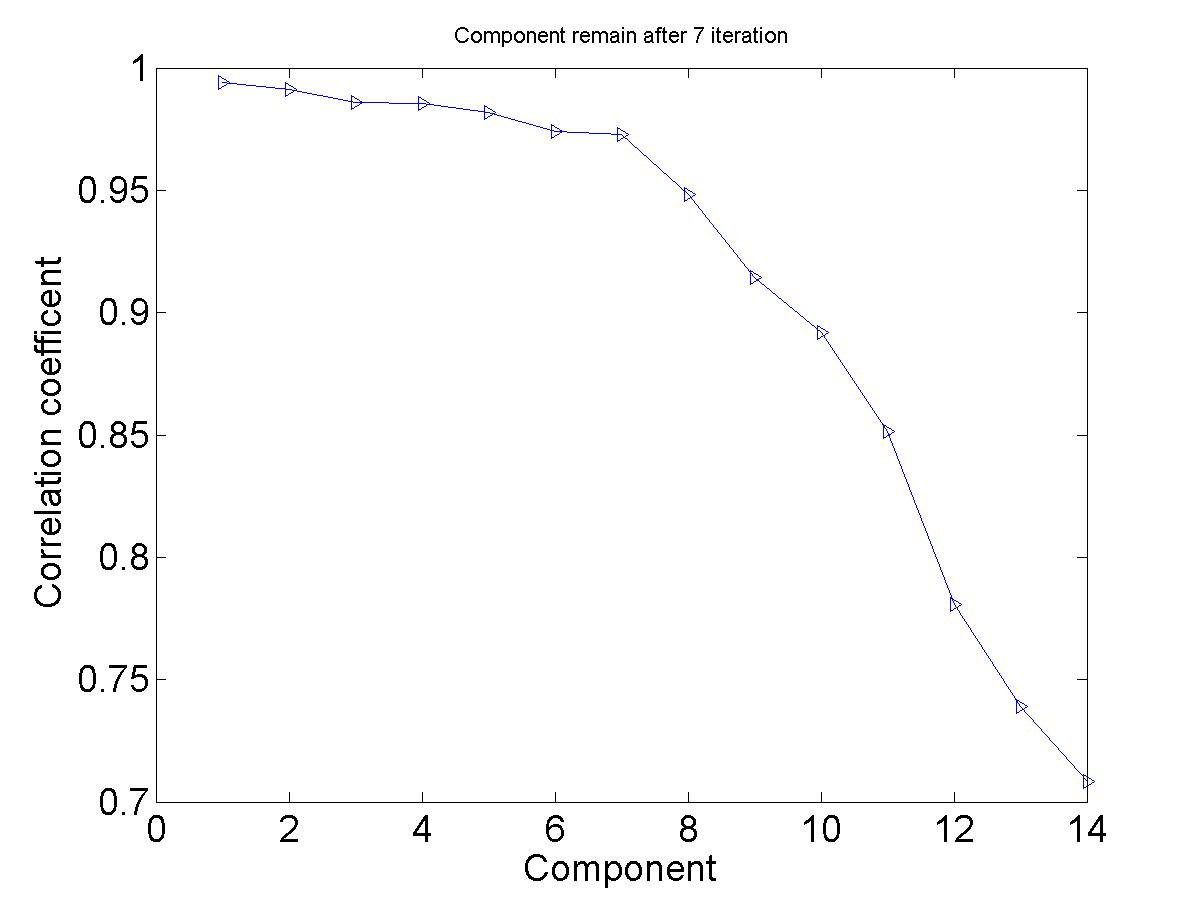
\includegraphics[width=.8\textwidth]{26.jpg}\\
\tiny{CCA results of the second data set}\label{toda2}
\endminipage\hfill
\end{figure}    
    
\end{frame}      
    
    
\begin{frame}{Outline of the process}

\begin{block}{\footnotesize{}}\tiny{}
\begin{enumerate} 
\vspace{0.05cm}
     \item \tiny{\textbf{\textit{Second dataset much higher level of artifacts compare to the first.}}}
     \item \tiny{\textbf{\textit{Semi automated CCA could be an fast approach}}}
     \item \tiny{\textbf{\textit{Visual perception is a vital for good performance}}}
     \item \tiny{\textbf{\textit{Recognition of low voltage and fast activities.}}}
     \item \tiny{\textbf{\textit{Some of the artifacts could not be suppressed with the CCA from the statistical nature of the method}}}
     \item \tiny{\textbf{\textit{Is still a subspace method where the resulting information is linearly approximated via consistently to the correlation values among channels and the CCA computed channels}}} 

     
\end{enumerate}
\end{block}

     
   
\end{frame} 
    
\begin{frame}{Differences between CCA and ICA}


\begin{block}{\footnotesize{}}\tiny{}
\begin{enumerate} 
\vspace{0.05cm}
     \item \tiny{\textbf{\textit{CCA is an straight forward implementation, ICA need to iteratively solve or optimize any parameter \cite{17}.}}} 
     \item \tiny{\textbf{\textit{In the ICA implementation there is no guarantee on the same output for identical data contrary to the CCA\cite{15}.}}} 
     \item \tiny{\textbf{\textit{CCA tries to uncorrelate  whereas ICA tries to independent the sources.}}} 
     \item \tiny{\textbf{\textit{CCA much faster compare to ICA}}}
     \item \tiny{\textbf{\textit{CCA claims better result compare to ICA}}} 
     \item \tiny{\textbf{\textit{ICA assumes the input data set to be full non-Gaussian CCA has no assumption}}} 
     \item \tiny{\textbf{\textit{ICA could be seen from different prospective.}}} 
     \item \tiny{\textbf{\textit{ICA in addition requires pre-processing  of the data, including here centering and whitening of the data.}}} 
     \item \tiny{\textbf{\textit{Auto-correlation is a well defined method thereby the correlation coefficient between the sources to be proceeded are defined very accurately in a very robust manner.}}} 

     
\end{enumerate}
\end{block}
     
   
\end{frame} 
    
    
    
    

\section{Nonlinear signal analysis}\label{Second-section}    
    
\begin{frame}{Nonlinear signal analysis}

\begin{figure}[!htbp]
\minipage{.5\textwidth}%
\centering
\includegraphics[width=.8\textwidth]{E1.jpg}\\
\tiny{DFA result of the control data set}\label{figa}
\endminipage\hfill
\minipage{.5\textwidth}%
\centering
\includegraphics[width=.8\textwidth]{E2.jpg}\\
\tiny{DFA result of the west data set}\label{figb}
\endminipage\hfill
\caption{\tiny Detrended fluctation analysis plots of the two data set}
\end{figure}
   
\end{frame}    
    
    
\begin{frame}{Non linear parameter estimation}

\begin{table}[!htbp]
\tiny
\centering
\begin{tabular}{ c c c c c c c c} 
\hline
$Control$&$1$&$2$&$3$&$4$&$5$&$\mu$&$\sigma$\\
\hline
$FD $&$1.7438$&$1.7298$&$1.7707$&$1.7208$&$1.7173$&$ 1.7365$&$ 4.7074e-04$\\
$1/f$&$-1.3486$&$-1.0308$&$-1.0754$&$-1.0624$&$-1.5117$&$-1.2058$&$ 0.0455$\\
$LE$&$0.0826$&$0.3860$&$0.2120$&$0.0825$&$0.0944$&$0.1938$&$0.0198$\\
$SampEnResults$&$2.3058$&$2.0164$&$2.0987$&$1.8646$&$2.1077$&$2.0786$&$0.0256$\\
&$0.6178$&$0.6472$&$0.7670$&$0.4271$&$0.5736$&$0.6065$&$0.0152$\\
\hline 
\end{tabular}
\end{table}



\begin{table}[!htbp]
\tiny
\centering
\begin{tabular}{ c c c c c c c c} 
\hline
$West$&$1$&$2$&$3$&$4$&$5$&$\mu$&$\sigma$\\
\hline
$FD$&$1.7448$&$1.5999$&$1.7198$&$1.7501$&$1.7059$&$ 1.7041$&$ 0.0037$\\
$1/f$&$-1.0898$&$-1.5659$&$-1.0138$&$-1.3829$&$-1.1288$&$-1.2362$&$ 0.0532$\\
$LE$&$0.1217$&$0.0878$&$0.2797$&$0.0807$&$0.3043$&$0.3222$&$0.0829$\\  
$SampEnResults$&$2.0307$&$2.2033$&$2.1825$&$2.1837$&$2.2467$&$2.1694$&$0.0067$\\
&$1.0327$&$0.6303$&$0.8739$&$0.5220$&$0.6609$&$ 0.7440$&$0.0423$\\
\hline 
\end{tabular}
\end{table}

\begin{table}[!htbp]
\tiny
\centering
\tiny Slope of the second part of line in DFA plots
\begin{tabular}{ c c c c c c c c} 
\hline
&$1$&$2$&$3$&$4$&$5$&$\mu$\\
\hline
$Control$&$31.4300$&$ 4.8353$&$4.8058$&$15.0472$&$21.1844$&$6.9868$\\
$West$&$6.9512$&$ 3.7947$&$0.7843$&$ 0.6201$&$13.9351$&$5.2171$\\
\hline 
\end{tabular}
\end{table}





\begin{table}[!htbp]
\tiny
\centering
\tiny Slope of the first part of line in DFA plots
\begin{tabular}{ c c c c c c c c} 
\hline
&$1$&$2$&$3$&$4$&$5$&$\mu$\\
\hline
$Control$&$129.5984$&$123.5662$&$132.5211$&$147.3374$&$127.0359$&$132.0118$\\
$West$&$137.6878$&$132.0872$&$135.5602$&$129.5709$&$135.0323$&$133.9877$\\
\hline 
\end{tabular}
\end{table}

   
\end{frame}    



\begin{frame}{DFA plots for both of the groups}

\begin{figure}[!htbp]
\minipage{.5\textwidth}%
\centering
\includegraphics[width=.7\textwidth]{E3.jpg}\\
\includegraphics[width=.7\textwidth]{E4.jpg}\\
\endminipage\hfill
\minipage{.5\textwidth}%
\centering
\includegraphics[width=.7\textwidth]{E8.jpg}\\
\includegraphics[width=.7\textwidth]{E9.jpg}\\
\endminipage\hfill
\end{figure}

    
\end{frame}

\begin{frame}{DFA plots for both of the groups.\textit{cont}}

\begin{figure}[!htbp]
\minipage{.5\textwidth}%
\centering
\includegraphics[width=.7\textwidth]{E5.jpg}\\
\includegraphics[width=.7\textwidth]{E6.jpg}\\
\endminipage\hfill
\minipage{.5\textwidth}%
\centering
\includegraphics[width=.7\textwidth]{E10.jpg}\\
\includegraphics[width=.7\textwidth]{E11.jpg}\\
\endminipage\hfill
\end{figure}

    
\end{frame}

\begin{frame}{DFA plots for both of the groups.\textit{cont I}}

\begin{figure}[!htbp]
\minipage{.5\textwidth}%
\centering
\includegraphics[width=.7\textwidth]{E7.jpg}\\
\endminipage\hfill
\minipage{.5\textwidth}%
\centering
\includegraphics[width=.7\textwidth]{E12.jpg}\\
\endminipage\hfill
\end{figure}

    
\end{frame}


\begin{frame}{F slope fitting}
\begin{figure}[!htbp]
\minipage{.5\textwidth}%
\centering
\includegraphics[width=.7\textwidth]{E33.jpg}\\
\includegraphics[width=.7\textwidth]{E34.jpg}\\
\endminipage\hfill
\minipage{.5\textwidth}%
\centering
\includegraphics[width=.7\textwidth]{E38.jpg}\\
\includegraphics[width=.7\textwidth]{E39.jpg}\\
\endminipage\hfill
\end{figure}
\end{frame}

\begin{frame}{F slope fitting \textit{cont}}
\begin{figure}[!htbp]
\minipage{.5\textwidth}%
\centering
\includegraphics[width=.7\textwidth]{E35.jpg}\\
\includegraphics[width=.7\textwidth]{E36.jpg}\\
\endminipage\hfill
\minipage{.5\textwidth}%
\centering
\includegraphics[width=.7\textwidth]{E40.jpg}\\
\includegraphics[width=.7\textwidth]{E41.jpg}\\
\endminipage\hfill
\end{figure}
\end{frame}

\begin{frame}{F slope fitting \textit{cont I}}
\begin{figure}[!htbp]
\minipage{.5\textwidth}%
\centering
\includegraphics[width=.7\textwidth]{E37.jpg}\\
\endminipage\hfill
\minipage{.5\textwidth}%
\centering
\includegraphics[width=.7\textwidth]{E42.jpg}\\
\endminipage\hfill
\end{figure}
\end{frame}



\begin{frame}{Discussion}


\begin{block}{\footnotesize{Scaling behaviour of the nonlinear system}}\tiny{}
\begin{enumerate} 
\vspace{0.05cm}
     \item \tiny{\textbf{\textit{FD evaluate the complexity degree of the signal. The rhythmic variation tends to decreases consequently FD in this case will be lower than normal subjects.}}}
     \item \tiny{\textbf{\textit{1/f slope indicates the smoothness of the time series. The values of abnormalities tends to be slightly lower compare to normal HR.}}} 
     \item \tiny{\textbf{\textit{DFA slope indicates the variability of the time series. It is composed of the short range $\alpha_{1}$ and long range $\alpha_{2}$. The slope is very low for very varying signals and slightly higher than 1 for rhythmically signals}}}
\end{enumerate}
\end{block}

\begin{block}{\footnotesize{Complexity and chaos of the system}}\tiny{}
\begin{enumerate} 
\vspace{0.05cm}
     \item \tiny{\textbf{\textit{LE defines the intensity of the chaotic behaviour and how much differ from periodic signals. Geometrically speaking defines the average rate of divergence of two trajectories. Positive values indicates a chaotic behaviour. It also outlines the sensitivity of the system to initial conditions together with a measurement of the predictability.}}}
     \item \tiny{\textbf{\textit{Sample entropy measures statistically the complexity and regularity of the time-series as well as its predictability.Its values are small when the HRV runs under same abnormalities and theoretically should be big when the HRV is normal.}}}

\end{enumerate}
\end{block}

\end{frame}

\begin{frame}{Comparison of the two groups}

\begin{block}{\footnotesize{}}\tiny{}
\begin{enumerate} 
\vspace{0.05cm}
     \item \tiny{\textbf{\textit{FD for the \textbf{\textit{Control}} case are fairly high, and there is no variation among the entities. In comparison to the \textbf{\textit{West}} the FD values are on average lower.}}}
     \item \tiny{\textbf{\textit{In the \textbf{\textit{Control}} data set this values on average tend to be lower compare to the \textbf{\textit{West}} data set although the difference is relatively small}}}
     \item \tiny{\textbf{\textit{DFA results on Control case it higher than the West set comparing respective individuate and therefore on average.}}}
     \item \tiny{\textbf{\textit{LE values \textbf{\textit{Control}} likewise the average are significantly smaller compare to the \textbf{\textit{West}} data set.}}}
     \item \tiny{\textbf{\textit{Mean value is however smaller in the \textbf{\textit{Control}} and therefore inferring some abnormalities compare to the \textbf{\textit{West}}.}}}
\end{enumerate}
\end{block}

\end{frame}



\emptyfooter
\begin{frame}{ }
\centering \textbf{\Large \textit{Thank you for your attention!}}
\begin{figure}[!htb]
\includegraphics[width=.3\textwidth]{QA.jpg}
\end{figure}
\largefooter
\end{frame}



\begin{frame}[allowframebreaks]
        \frametitle{References}
        \nocite{*}
        \bibliography{Bibl}
        \bibliographystyle{plain}
\end{frame}

\end{document}